\documentclass[aspectratio=169,10pt,t]{beamer}

\usepackage[T1]{fontenc}
\usepackage[utf8]{inputenc}
\usepackage[french]{babel}
\usepackage{lmodern}
\usepackage{microtype}
\usepackage{amsmath,amssymb,bm}
\usepackage{graphicx}
\usepackage{booktabs}
\usepackage{tabularx}
\usepackage{ragged2e}
\usepackage{tikz}
\usetikzlibrary{arrows.meta,positioning,calc,shapes.geometric,decorations.pathmorphing}
\usetheme{Copenhagen}

% -----------------------------------------------------------------------------
% Identité visuelle reprise du modèle Frost / CentraleSupélec.
% -----------------------------------------------------------------------------
\definecolor{bordeauCS}{RGB}{132,29,59}
\definecolor{grisCS}{RGB}{114,104,128}
\definecolor{PressureBlue}{RGB}{42,111,151}
\definecolor{HomStrainPurple}{RGB}{104,82,148}
\definecolor{InhomStrainGreen}{RGB}{35,123,103}

% Alias sémantiques utilisés dans les schémas existants.
\colorlet{CSOrange}{bordeauCS}
\colorlet{DeepNavy}{black!82}
\colorlet{Teal}{grisCS}
\colorlet{WarmGold}{bordeauCS!55!white}
\colorlet{Ink}{black!82}
\colorlet{Slate}{grisCS}
\colorlet{Mist}{grisCS!9!white}
\colorlet{PaleOrange}{bordeauCS!9!white}
\colorlet{PaleTeal}{grisCS!10!white}
\colorlet{PaleGold}{bordeauCS!4!white}
\colorlet{PalePressure}{PressureBlue!9!white}

\setbeamercolor{normal text}{fg=Ink,bg=white}
\setbeamercolor{palette primary}{bg=bordeauCS,fg=white}
\setbeamercolor{palette secondary}{bg=grisCS,fg=white}
\setbeamercolor{palette tertiary}{bg=bordeauCS,fg=white}
\setbeamercolor{palette quaternary}{bg=grisCS,fg=white}
\setbeamercolor{structure}{fg=grisCS}
\setbeamercolor{section in head/foot}{bg=grisCS,fg=white}
\setbeamercolor{subsection in head/foot}{bg=bordeauCS,fg=white}
\setbeamercolor{frametitle}{bg=bordeauCS,fg=white}
\setbeamercolor{author in head/foot}{bg=grisCS,fg=white}
\setbeamercolor{title in head/foot}{bg=bordeauCS,fg=white}
\setbeamercolor{date in head/foot}{bg=grisCS,fg=white}
\setbeamercolor{progress bar}{bg=grisCS!18!white,fg=bordeauCS}
\setbeamercolor{title}{fg=bordeauCS}
\setbeamercolor{subtitle}{fg=Slate}
\setbeamercolor{alerted text}{fg=bordeauCS}
\setbeamercolor{block title}{fg=white,bg=bordeauCS}
\setbeamercolor{block body}{fg=Ink,bg=Mist}
\setbeamercolor{example text}{fg=grisCS}

\setbeamerfont{normal text}{size=\fontsize{10.0}{11.8}}
\setbeamerfont{title}{series=\bfseries,size=\fontsize{23}{26}}
\setbeamerfont{subtitle}{size=\fontsize{14}{17}}
\setbeamerfont{frametitle}{series=\bfseries,size=\fontsize{17.5}{20}}
\setbeamerfont{block title}{series=\bfseries,size=\fontsize{10.5}{12}}
\setbeamerfont{block body}{size=\fontsize{9.6}{11.4}}

\setbeamersize{text margin left=0.66cm,text margin right=0.66cm}
\beamertemplatenavigationsymbolsempty
\setbeamertemplate{itemize item}{\color{CSOrange}\raise0.15ex\hbox{\rule{0.52ex}{0.52ex}}}
\setbeamertemplate{itemize subitem}{\color{Teal}\raise0.2ex\hbox{\scriptsize$\blacktriangleright$}}
\setbeamertemplate{enumerate item}{\color{CSOrange}\bfseries\insertenumlabel.}
\setlength{\leftmargini}{1.25em}
\setlength{\leftmarginii}{1.15em}

\makeatletter
\setbeamertemplate{footline}{%
  \leavevmode%
  \hbox{%
    \begin{beamercolorbox}[wd=.30\paperwidth,ht=2.25ex,dp=1ex,center]{author in head/foot}%
      \usebeamerfont{author in head/foot}\insertshortauthor
    \end{beamercolorbox}%
    \begin{beamercolorbox}[wd=.40\paperwidth,ht=2.25ex,dp=1ex,center]{title in head/foot}%
      \usebeamerfont{title in head/foot}\insertshorttitle
    \end{beamercolorbox}%
    \begin{beamercolorbox}[wd=.30\paperwidth,ht=2.25ex,dp=1ex,right]{date in head/foot}%
      \usebeamerfont{date in head/foot}\insertshortdate{}\hspace*{2em}%
      \insertframenumber{} / \inserttotalframenumber\hspace*{2ex}
    \end{beamercolorbox}%
  }\vskip0pt%
}
\addtobeamertemplate{footline}{%
  \nointerlineskip
  \begin{beamercolorbox}[wd=\paperwidth,ht=2pt,dp=0pt]{progress bar}%
    \color{bordeauCS}\rule{\dimexpr\paperwidth*\insertframenumber/\inserttotalframenumber\relax}{2pt}%
  \end{beamercolorbox}%
}{}
% Beamer réinitialise la transition au début de chaque page physique. On
% l'applique juste avant l'analyse du titre afin de préserver le gabarit.
\patchcmd{\beamer@frameslide}
  {\beamer@checkframetitle}
  {\beamer@dotrans[{duration=0.15}]{Fade}\beamer@checkframetitle}
  {}{}
\makeatother

\newcommand{\source}[1]{%
  \par\vspace{0.12cm}{\color{Slate}\fontsize{6.6}{7.8}\selectfont Source : #1\par}%
}
\newcommand{\takeaway}[1]{%
  \begin{beamercolorbox}[wd=\linewidth,rounded=true,sep=0.56em]{block body}
    \centering\bfseries\color{DeepNavy}#1
  \end{beamercolorbox}
}
\newcommand{\metric}[3][CSOrange]{%
  \begin{beamercolorbox}[wd=\linewidth,rounded=true,sep=0.48em]{block body}
    \centering{\color{#1}\bfseries\fontsize{16.5}{18.5}\selectfont #2}\par
    \vspace{0.08cm}{\color{Ink}\fontsize{8.9}{10.5}\selectfont #3}
  \end{beamercolorbox}
}
\newcommand{\compactmetric}[3][CSOrange]{%
  \begin{beamercolorbox}[wd=\linewidth,rounded=true,sep=0.24em]{block body}
    \centering{\color{#1}\bfseries\fontsize{13.2}{14.4}\selectfont #2}\par
    \vspace{0.02cm}{\color{Ink}\fontsize{8.0}{9.0}\selectfont #3}
  \end{beamercolorbox}
}
\newcommand{\tagline}[2]{\textcolor{#1}{\bfseries #2}}

\graphicspath{{assets/}}
\hypersetup{
  colorlinks=true,
  urlcolor=Teal,
  linkcolor=CSOrange
}

% Accès discret à la slide finale de questions depuis toutes les slides de
% contenu. Le test sur le compteur exclut la page de titre et le sommaire.
\newif\ifdiscussionbuttonenabled
\discussionbuttonenabledtrue
\newcommand{\discussionbutton}{%
  \ifdiscussionbuttonenabled
    \ifnum\value{framenumber}>2\relax
      \begin{tikzpicture}[remember picture,overlay]
        \node[anchor=south east,inner sep=0pt]
          at ([xshift=-0.18cm,yshift=0.48cm]current page.south east) {%
            \hyperlink{questions-discussion}{%
              \tikz[baseline=-0.5ex]{%
                \path[fill=grisCS!22!white,draw=grisCS!38!white,line width=0.20pt,
                  rounded corners=0.6pt]
                  (0,0) rectangle (0.20cm,0.14cm);%
              }%
            }%
          };
      \end{tikzpicture}%
    \fi
  \fi
}
% Fondu très bref entre les pages pour adoucir le rafraîchissement du lecteur.
\addtobeamertemplate{background canvas}{}{\discussionbutton}

\title[Transitions quantiques et susceptibilité]{Transitions de phase quantiques \& susceptibilité diélectrique dans les paraélectriques quantiques }
\subtitle{Application à \texorpdfstring{$\mathrm{BaTiO}_3$ et $\mathrm{Ba}_x\mathrm{Sr}_{1-x}\mathrm{TiO}_3$}{BaTiO3 et BaxSr1-xTiO3}}
\author[M. Devin-Pinson]{Maxime DEVIN-PINSON}
\institute{Stage 3A --- Laboratoire SPMS, UMR 8580, CentraleSupélec}
\date[22/09/2026]{Soutenance finale --- 22 septembre 2026 à 13\,h\,30}

\begin{document}

% =============================================================================
% OUVERTURE ET CONTEXTE
% =============================================================================

\begin{frame}[plain]
  \vspace{0.34cm}
  \begin{beamercolorbox}[wd=\textwidth,rounded=true,sep=0.82em,center]{frametitle}
    {\bfseries\fontsize{19.5}{22.5}\selectfont\inserttitle\par}
  \end{beamercolorbox}
  \vspace{0.34cm}
  {\centering\color{grisCS}\fontsize{13.2}{15.8}\selectfont
    \insertsubtitle\par}
  \vfill
  {\centering\color{Ink}\bfseries\fontsize{14}{16}\selectfont
    \insertauthor\par}
  \vspace{0.14cm}
  {\centering\color{Slate}\fontsize{9.7}{11.5}\selectfont
    \insertinstitute\par}
  \vspace{0.20cm}
  {\centering\color{Ink}\fontsize{11}{13}\selectfont
    \insertdate\par}
  \vspace{0.38cm}
  \centering
  {\color{bordeauCS}\rule{0.30\paperwidth}{2.2pt}}%
  {\color{grisCS}\rule{0.08\paperwidth}{2.2pt}}
  \begin{tikzpicture}[remember picture,overlay]
    \node[anchor=south west,inner sep=0pt]
      at ([xshift=0.58cm,yshift=0.16cm]current page.south west)
      {
\includegraphics[width=2.45cm]{logo_cs.png}};
    \node[anchor=south east,inner sep=0pt]
      at ([xshift=-0.58cm,yshift=0.16cm]current page.south east)
      {
\includegraphics[width=3.75cm,trim=70 60 70 40,clip]{logo_spms.png}};
  \end{tikzpicture}
  \vspace{0.05cm}
\end{frame}

\begin{frame}{Sommaire --- les cinq parties de l'exposé}
  \centering
  \vspace{0.20cm}
  \begin{tikzpicture}[
      node distance=0.20cm,
      stepbox/.style={rounded corners=2pt,minimum width=2.28cm,minimum height=1.26cm,align=center,font=\small\bfseries,text=DeepNavy},
      arr/.style={-{Latex[length=2.2mm]},thick,Slate}
    ]
    \node[stepbox,fill=PaleOrange] (s1) {Besoin et\\matériau};
    \node[stepbox,fill=Mist,right=of s1] (s2) {Hamiltonien\\effectif};
    \node[stepbox,fill=PaleTeal,right=of s2] (s3) {Passage continu\\et quantique};
    \node[stepbox,fill=PaleGold,right=of s3] (s4) {Résolution et\\contrôles};
    \node[stepbox,fill=PaleOrange,right=of s4] (s5) {Résultats, limites\\et suites};
    \draw[arr] (s1)--(s2); \draw[arr] (s2)--(s3); \draw[arr] (s3)--(s4); \draw[arr] (s4)--(s5);
    \foreach \n/\lab/\c in {s1/1/CSOrange,s2/2/DeepNavy,s3/3/Teal,s4/4/WarmGold,s5/5/CSOrange}{
      \node[circle,fill=\c,text=white,font=\bfseries,minimum size=0.60cm,above=0.18cm of \n] {\lab};
    }
  \end{tikzpicture}
  \vspace{0.72cm}
  \begin{columns}[T,onlytextwidth]
    \column{0.46\textwidth}
      \tagline{CSOrange}{Question scientifique}

      Comment les fluctuations thermiques et quantiques renormalisent-elles la
      réponse $\bm\chi(T)$ qui relie le champ $\bm E$ à la polarisation $\bm P$ ?
    \column{0.50\textwidth}
      \tagline{Teal}{Question d'ingénierie}

      Comment garder une chaîne de calcul traçable, stable numériquement, reproductible et confrontable aux mesures ?
  \end{columns}
\end{frame}

\iffalse
\begin{frame}{Dictionnaire des termes et grandeurs utilisés}
  \small
  \renewcommand{\arraystretch}{1.18}
  \begin{tabular}{@{}>{\RaggedRight\arraybackslash\bfseries\color{DeepNavy}}m{0.20\linewidth}
    >{\RaggedRight\arraybackslash}m{0.75\linewidth}@{}}
    \toprule
    Symbole & \bfseries\color{DeepNavy} Interprétation \\
    \midrule
    $\bm u_i$ & amplitude locale du mode mou dans la maille $i$ \\
    $\bm P$ & polarisation ionique, $\bm P=\bm\chi\,\bm E$ en unités gaussiennes \\
    $\bm A(\bm k,\omega_n;T)$ & matrice de rigidité renormalisée du champ de polarisation \\
    $\bar{\bm G}$ & covariance des fluctuations, intégrée sur la zone de Brillouin \\
    1ZB & première zone de Brillouin : cellule élémentaire de l'espace réciproque, espace des $\bm k$ \\
    $\bm\chi$ & réponse gaussienne statique, $\bm\chi=\Omega_0\bm A^{-1}(\bm 0,0;T)$ \\
    $\varepsilon_r$ & permittivité relative, $\varepsilon_r=\varepsilon_\infty+4\pi\chi_T$ en unités gaussiennes \\
    DFT & théorie de la fonctionnelle de la densité \\
    SCHA & approximation harmonique auto-cohérente \\
    \bottomrule
  \end{tabular}
\end{frame}
\fi

\section{Contexte et besoin}

{
\setbeamerfont{frametitle}{series=\bfseries,size=\fontsize{16.5}{19}}
\begin{frame}[label=qa-app]{Le BST peut accorder un circuit micro-ondes par tension}
  \begin{columns}[c,onlytextwidth]
    \column{0.26\textwidth}
      \centering
      {\color{DeepNavy}\bfseries\fontsize{13.8}{16.2}\selectfont
        $V_{\rm DC}$\par}
      {\color{CSOrange}\fontsize{15}{17}\selectfont$\Downarrow$\par}
      {\color{DeepNavy}\bfseries\fontsize{12.8}{15.0}\selectfont
        $\varepsilon_r(E_{\rm DC})$\par}
      {\color{CSOrange}\fontsize{15}{17}\selectfont$\Downarrow$\par}
      {\color{DeepNavy}\bfseries\fontsize{12.2}{14.4}\selectfont
        $f_0$ ou phase $\varphi$\par}

    \column{0.29\textwidth}
      \centering
      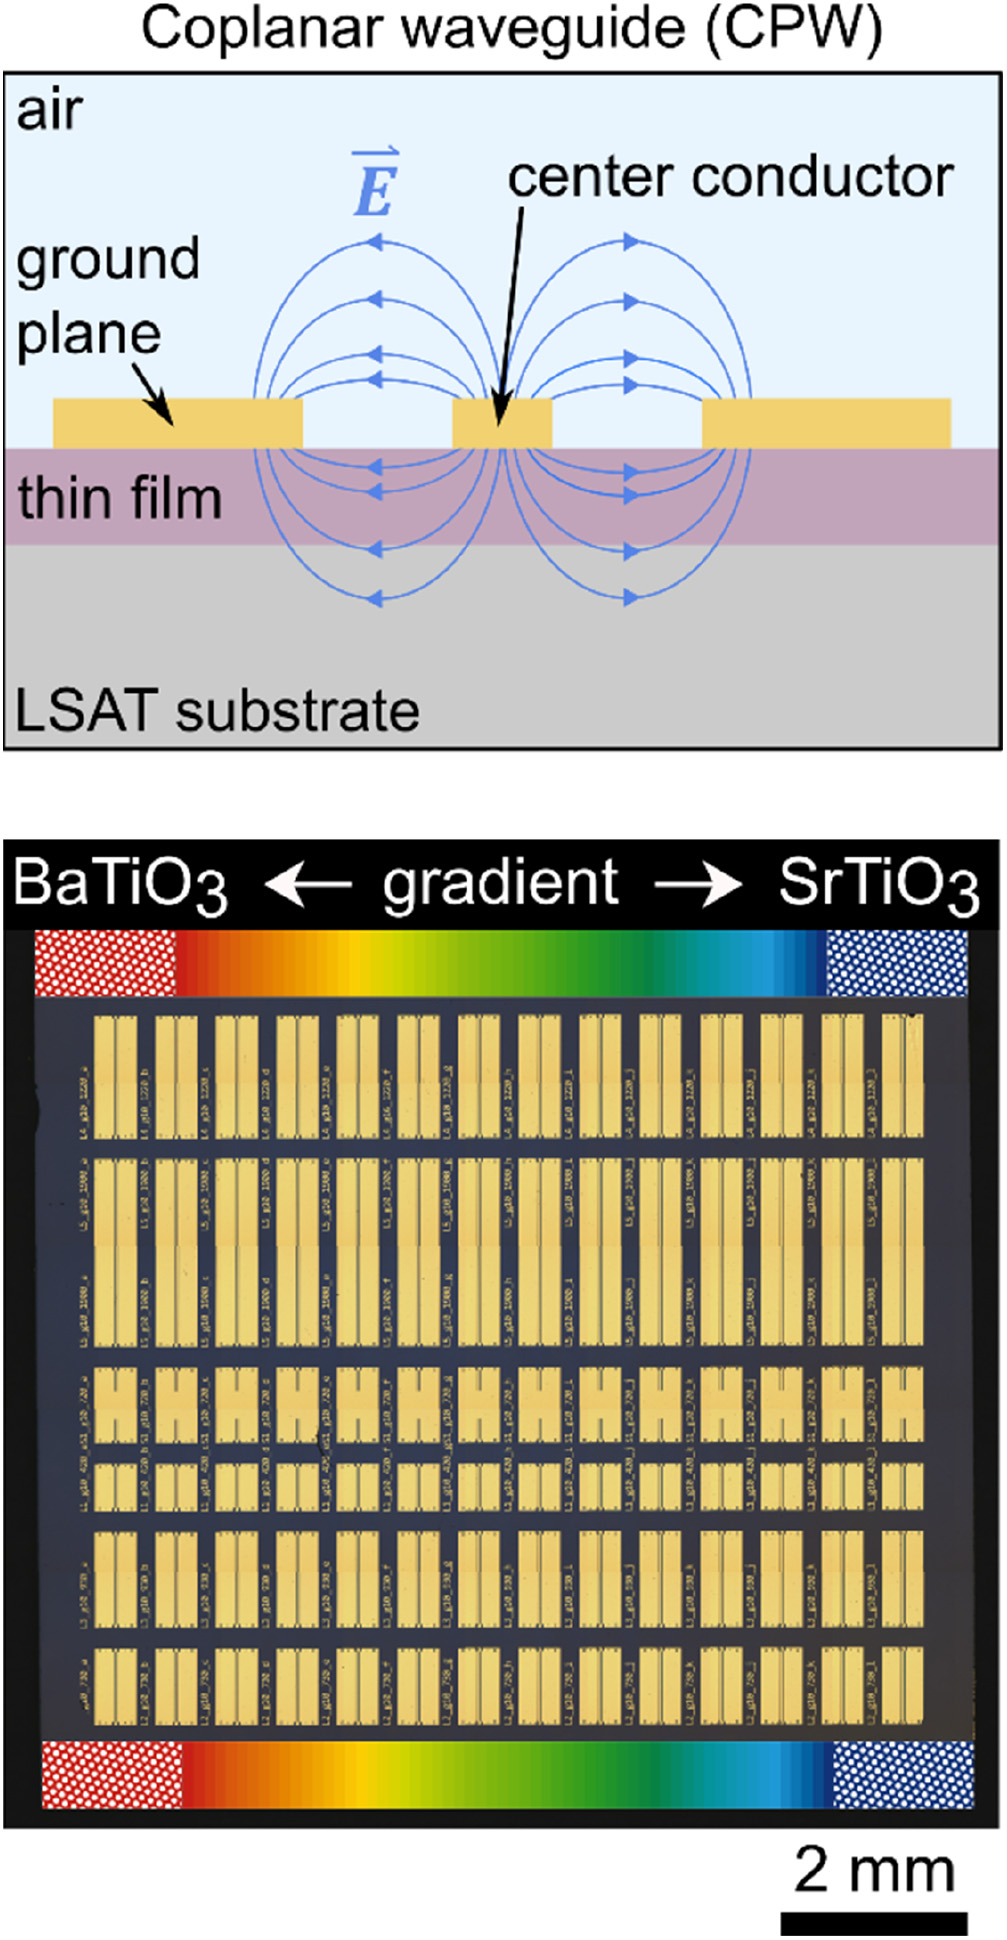
\includegraphics[height=2.70cm,trim=0 1120 0 0,clip]
        {applications/bst_cpw_marksz.png}
      \vspace{0.04cm}

      {\color{Slate}\fontsize{6.8}{7.9}\selectfont
        Guide coplanaire : le champ traverse le film BST.\par}

    \column{0.39\textwidth}
      \centering
      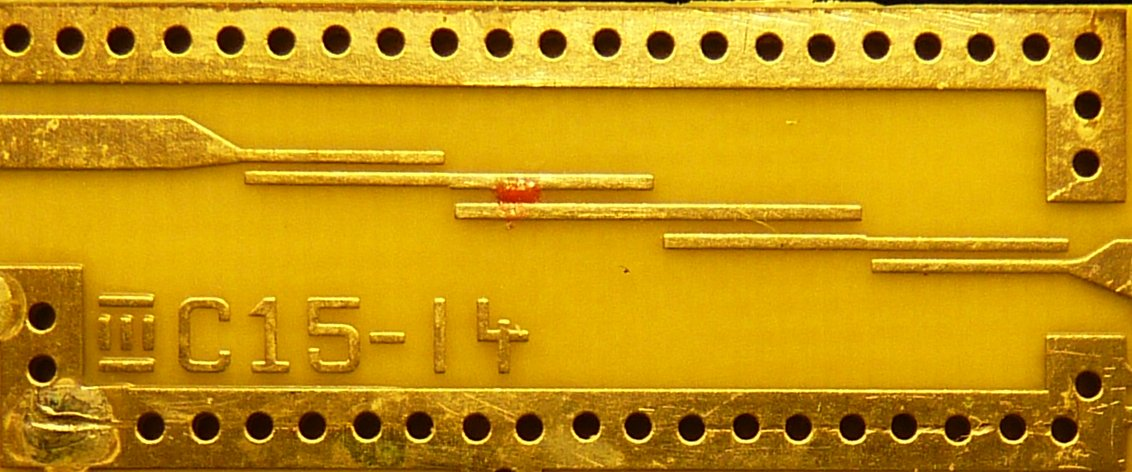
\includegraphics[width=\linewidth]{applications/microstrip_bandpass_filter.jpg}
      \vspace{0.05cm}

      {\color{Slate}\fontsize{6.8}{7.9}\selectfont
        Filtre passe-bande micro-ruban à résonateurs $\lambda/2$.\par}
  \end{columns}

  \vspace{0.22cm}
  \begin{columns}[T,onlytextwidth]
    \column{0.28\textwidth}
      \centering
      \tagline{Teal}{BST sans plomb}
    \column{0.36\textwidth}
      \centering
      {\color{DeepNavy}\bfseries
        Ba/Sr $\Longrightarrow T_C$ $\Longrightarrow$ sensibilité}
    \column{0.30\textwidth}
      \centering
      \tagline{CSOrange}{Filtre --- résonateur --- déphaseur}
  \end{columns}
  \source{schéma CPW : Marksz et al., \textit{Phys. Rev. Applied} 15, 064061 (2021) ; photo : Catslash, Wikimedia Commons, domaine public ; principe BST : Tagantsev et al. (2003).}
\end{frame}
}

\begin{frame}{Deux pistes où la forte permittivité devient utile}
  \begin{columns}[T,onlytextwidth]
    \column{0.47\textwidth}
      \centering
      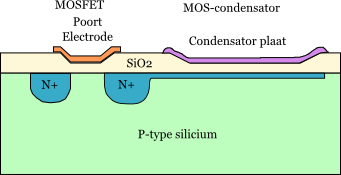
\includegraphics[height=1.78cm]{applications/dram_1t1c.png}
      \vspace{0.04cm}

      {\color{Slate}\fontsize{7.2}{8.4}\selectfont Une cellule : 1 transistor + 1 condensateur.\par}
      \vspace{0.18cm}
      \tagline{Teal}{Mémoire vive DRAM}\par
      \vspace{0.10cm}
      {\color{Teal}\bfseries\fontsize{18}{20}\selectfont
        $\varepsilon_r\!\uparrow\quad\Longrightarrow\quad A\!\downarrow$\par}
      \vspace{0.10cm}
      Stocker une charge sur une \textbf{surface plus petite}.\par
      \vspace{0.10cm}
      {\bfseries BST : diélectrique candidat.}
    \column{0.47\textwidth}
      \centering
      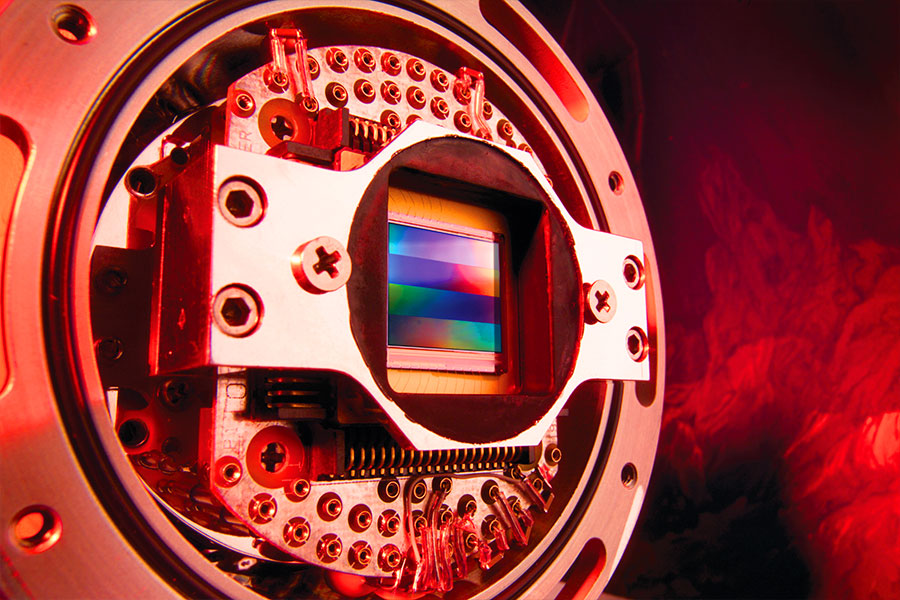
\includegraphics[height=1.78cm]{applications/ir_focal_plane_array.jpg}
      \vspace{0.04cm}

      {\color{Slate}\fontsize{7.2}{8.4}\selectfont Exemple de matrice infrarouge non refroidie, JPL/NASA.\par}
      \vspace{0.18cm}
      \tagline{WarmGold}{Détection infrarouge}\par
      \vspace{0.10cm}
      {\color{WarmGold}\bfseries\fontsize{18}{20}\selectfont
        $\Delta T\ \longrightarrow\ \Delta P\ \longrightarrow\ Q$\par}
      \vspace{0.10cm}
      Convertir un écart de température en \textbf{signal électrique}.\par
      \vspace{0.10cm}
      {\bfseries BST : matériau pyroélectrique candidat.}
  \end{columns}
  \vspace{0.16cm}
  \source{Ezhilvalavan et Tseng (2000) ; Liu et al. (2002) ; schéma DRAM : Livinus, CC BY-SA 4.0 ; photo : JPL/NASA.}
\end{frame}

\begin{frame}{Les familles polaires s'imbriquent au sein des isolants}
  \centering
  \begin{tikzpicture}[x=1cm,y=1cm,
      topbox/.style={rounded corners=2pt,minimum width=3.10cm,minimum height=0.72cm,
        align=center,text=DeepNavy,font=\fontsize{8.3}{9.7}\selectfont},
      label/.style={font=\bfseries\fontsize{8.1}{9.5}\selectfont,text=DeepNavy},
      small/.style={font=\fontsize{6.8}{8.0}\selectfont,text=Slate,align=center}]

    % Premier niveau : transport des charges.
    \node[topbox,fill=PaleOrange] (cond) at (1.75,5.18)
      {\bfseries CONDUCTEURS\\[-0.03cm]{\fontsize{6.7}{7.8}\selectfont charges mobiles --- Cu, Al}};
    \node[topbox,fill=Mist] (semi) at (6.00,5.18)
      {\bfseries SEMI-CONDUCTEURS\\[-0.03cm]{\fontsize{6.7}{7.8}\selectfont conductivité contrôlée --- Si}};
    \node[topbox,fill=PaleTeal] (isol) at (10.25,5.18)
      {\bfseries ISOLANTS\\[-0.03cm]{\fontsize{6.7}{7.8}\selectfont charges liées --- céramiques}};
    \draw[-{Latex[length=2.2mm]},thick,Slate] (cond.east) -- (semi.west);
    \draw[-{Latex[length=2.2mm]},thick,Slate] (semi.east) -- (isol.west);
    \node[font=\fontsize{6.5}{7.5}\selectfont\bfseries,text=Slate]
      at (6.00,5.72) {conductivité décroissante};

    % Toutes les familles polaires sont rangées dans l'ensemble des isolants.
    \draw[-{Latex[length=2.2mm]},thick,Slate] (isol.south) -- (10.25,4.52);
    \draw[rounded corners=4pt,draw=Teal,line width=1.0pt,fill=PaleTeal]
      (0.20,0.18) rectangle (11.80,4.50);
    \node[anchor=west,label] at (0.48,4.20) {DANS LES ISOLANTS};
    \node[anchor=east,font=\bfseries\fontsize{7.1}{8.3}\selectfont,text=CSOrange]
      at (11.52,4.20) {$\mathrm{BaTiO}_3$ et BST : branche fixée par $x$ et $T$};

    \draw[rounded corners=3pt,draw=Slate,line width=0.9pt,fill=white]
      (0.50,0.48) rectangle (11.50,3.86);
    \node[anchor=west,label] at (0.78,3.56)
      {DIÉLECTRIQUES : isolants polarisables sous un champ $E$};

    % Branche sans polarisation spontanée.
    \draw[rounded corners=3pt,draw=Teal,line width=0.9pt,fill=Mist]
      (0.84,0.82) rectangle (5.18,3.18);
    \node[label,text=Teal] at (3.01,2.86) {PARAÉLECTRIQUES};
    \node[small] at (3.01,2.52) {$P=0$ sans champ};
    \draw[rounded corners=2pt,draw=Teal,line width=0.8pt,fill=PaleTeal]
      (1.20,1.10) rectangle (4.82,2.16);
    \node[font=\bfseries\fontsize{6.8}{7.5}\selectfont,text=Teal,align=center]
      at (3.01,1.82) {PARAÉLECTRIQUES\\[-0.04cm]QUANTIQUES};
    \node[font=\fontsize{6.1}{7.1}\selectfont,text=Slate,align=center]
      at (3.01,1.36) {point zéro $\Rightarrow$ transition évitée};

    % Branche emboîtée : piézo > pyro > ferro.
    \draw[rounded corners=3pt,draw=CSOrange,line width=0.9pt,fill=PaleOrange]
      (5.52,0.82) rectangle (11.16,3.18);
    \node[label,text=CSOrange] at (8.34,2.86) {PIÉZOÉLECTRIQUES};
    \node[small] at (8.34,2.53) {déformation $\leftrightarrow$ tension};
    \draw[rounded corners=2pt,draw=WarmGold,line width=0.8pt,fill=white]
      (6.02,1.08) rectangle (10.66,2.30);
    \node[font=\bfseries\fontsize{7.5}{8.7}\selectfont,text=WarmGold]
      at (8.34,2.02) {PYROÉLECTRIQUES};
    \node[small] at (8.34,1.72) {$\Delta T\longrightarrow\Delta P$};
    \draw[rounded corners=2pt,draw=CSOrange,line width=0.8pt,fill=PaleOrange]
      (6.42,1.16) rectangle (10.26,1.58);
    \node[font=\bfseries\fontsize{6.4}{7.4}\selectfont,text=CSOrange]
      at (8.34,1.37) {FERROÉLECTRIQUES : $P_{\rm s}\neq0$};
  \end{tikzpicture}
\end{frame}

\begin{frame}{Mon stage en une phrase}
  \begin{columns}[T,onlytextwidth]
    \column{0.64\textwidth}
      {\color{DeepNavy}\bfseries\fontsize{17}{20}\selectfont Construire une chaîne traçable entre la physique atomique et une grandeur mesurable.\par}
      \vspace{0.22cm}
      \begin{itemize}[<+->]\setlength\itemsep{0.22cm}
        \item \textbf{Besoin de l'équipe :} interpréter et anticiper la réponse diélectrique de pérovskites ferroélectriques.
        \item \textbf{Ma mission :} transformer un Hamiltonien paramétré par DFT\textsuperscript{*} en un modèle continu quantique, puis en un solveur de $\chi(T)$.
        \item \textbf{Critère de réussite :} une méthode compréhensible, reproductible et confrontable aux mesures.
      \end{itemize}
    \column{0.32\textwidth}
      \begin{beamercolorbox}[rounded=true,sep=0.75em]{block body}
        \tagline{CSOrange}{Structure d'accueil}\par
        Laboratoire SPMS\par
        CentraleSupélec, Saclay

        \vspace{0.24cm}
        \tagline{Teal}{Encadrement scientifique}\par
        Igor Kornev

        \vspace{0.24cm}
        \tagline{WarmGold}{Encadrement institutionnel}\par
        Pierre-Eymeric Janolin
      \end{beamercolorbox}
  \end{columns}
  \uncover<2->{%
    \begin{tikzpicture}[remember picture,overlay]
      \node[anchor=south east,font=\fontsize{6.5}{7.5}\selectfont\itshape,text=Slate]
        at ([xshift=-0.42cm,yshift=0.34cm]current page.south east)
        {\textsuperscript{*}Théorie de la fonctionnelle de la densité};
    \end{tikzpicture}%
  }
\end{frame}

\begin{frame}{Relier quatre échelles impose une méthode traçable}
  \centering
  \begin{tikzpicture}[
      node distance=0.45cm,
      flowbox/.style={rounded corners=2pt,minimum width=2.65cm,minimum height=1.18cm,align=center,font=\bfseries,draw=none},
      arr/.style={-{Latex[length=2.7mm]},very thick,Slate}
    ]
    \node[flowbox,fill=PaleOrange,text=DeepNavy] (dft) {Paramètres\\\textit{ab initio}};
    \node[flowbox,fill=Mist,text=DeepNavy,right=of dft] (lat) {Hamiltonien\\sur le réseau};
    \node[flowbox,fill=PaleTeal,text=DeepNavy,right=of lat] (field) {Théorie continue\\+ quantique};
    \node[flowbox,fill=PaleGold,text=DeepNavy,right=of field] (obs) {Observable\\$\chi(T)$};
    \draw[arr] (dft) -- (lat);
    \draw[arr] (lat) -- (field);
    \draw[arr] (field) -- (obs);
    \node[Slate,font=\small,below=0.12cm of dft] {$Z^*$, forces, élasticité};
    \node[Slate,font=\small,below=0.12cm of lat] {$\bm u_i$, interactions};
    \node[Slate,font=\small,below=0.12cm of field]
      {$\bm P(\bm r,\tau)$, SCHA\textsuperscript{*}};
    \node[Slate,font=\small,below=0.12cm of obs] {comparaison aux mesures};
  \end{tikzpicture}

  \vspace{0.48cm}
  \begin{columns}[T,onlytextwidth]
    \column{0.31\textwidth}
      \tagline{CSOrange}{FIDÉLITÉ PHYSIQUE}\par
      \vspace{0.08cm}
      Paramètres DFT publiés ; noyaux complets ; déformations homogènes et inhomogènes séparées.
    \column{0.31\textwidth}
      \tagline{Teal}{CALCUL DÉTERMINISTE}\par
      \vspace{0.08cm}
      Quadrature de la zone de Brillouin ; sommes quantiques analytiques ; racines encadrées.
    \column{0.31\textwidth}
      \tagline{WarmGold}{TRAÇABILITÉ}\par
      \vspace{0.08cm}
      Hypothèses et unités explicites ; stabilité, convergence et origine des écarts contrôlées.
  \end{columns}
  \vspace{0.30cm}
  \begin{beamercolorbox}[wd=\linewidth,rounded=true,sep=0.46em]{block body}
    \centering\color{DeepNavy}\bfseries
    Périmètre : modèle semi-analytique --- ni Monte-Carlo ni dynamique moléculaire.
  \end{beamercolorbox}
  \begin{tikzpicture}[remember picture,overlay]
    \node[anchor=south east,font=\fontsize{6.5}{7.5}\selectfont\itshape,text=Slate]
      at ([xshift=-0.42cm,yshift=0.34cm]current page.south east)
      {\textsuperscript{*}Approximation harmonique auto-cohérente};
  \end{tikzpicture}
  \vspace{-0.22cm}
\end{frame}

\begin{frame}[label=qa-quantum]{Pourquoi faut-il intégrer les fluctuations quantiques ?}
  \begin{columns}[T,onlytextwidth]
    \column{0.56\textwidth}
      \centering
      \tagline{CSOrange}{Mesure réelle sur SrTiO$_3$}\par
      \vspace{0.04cm}
      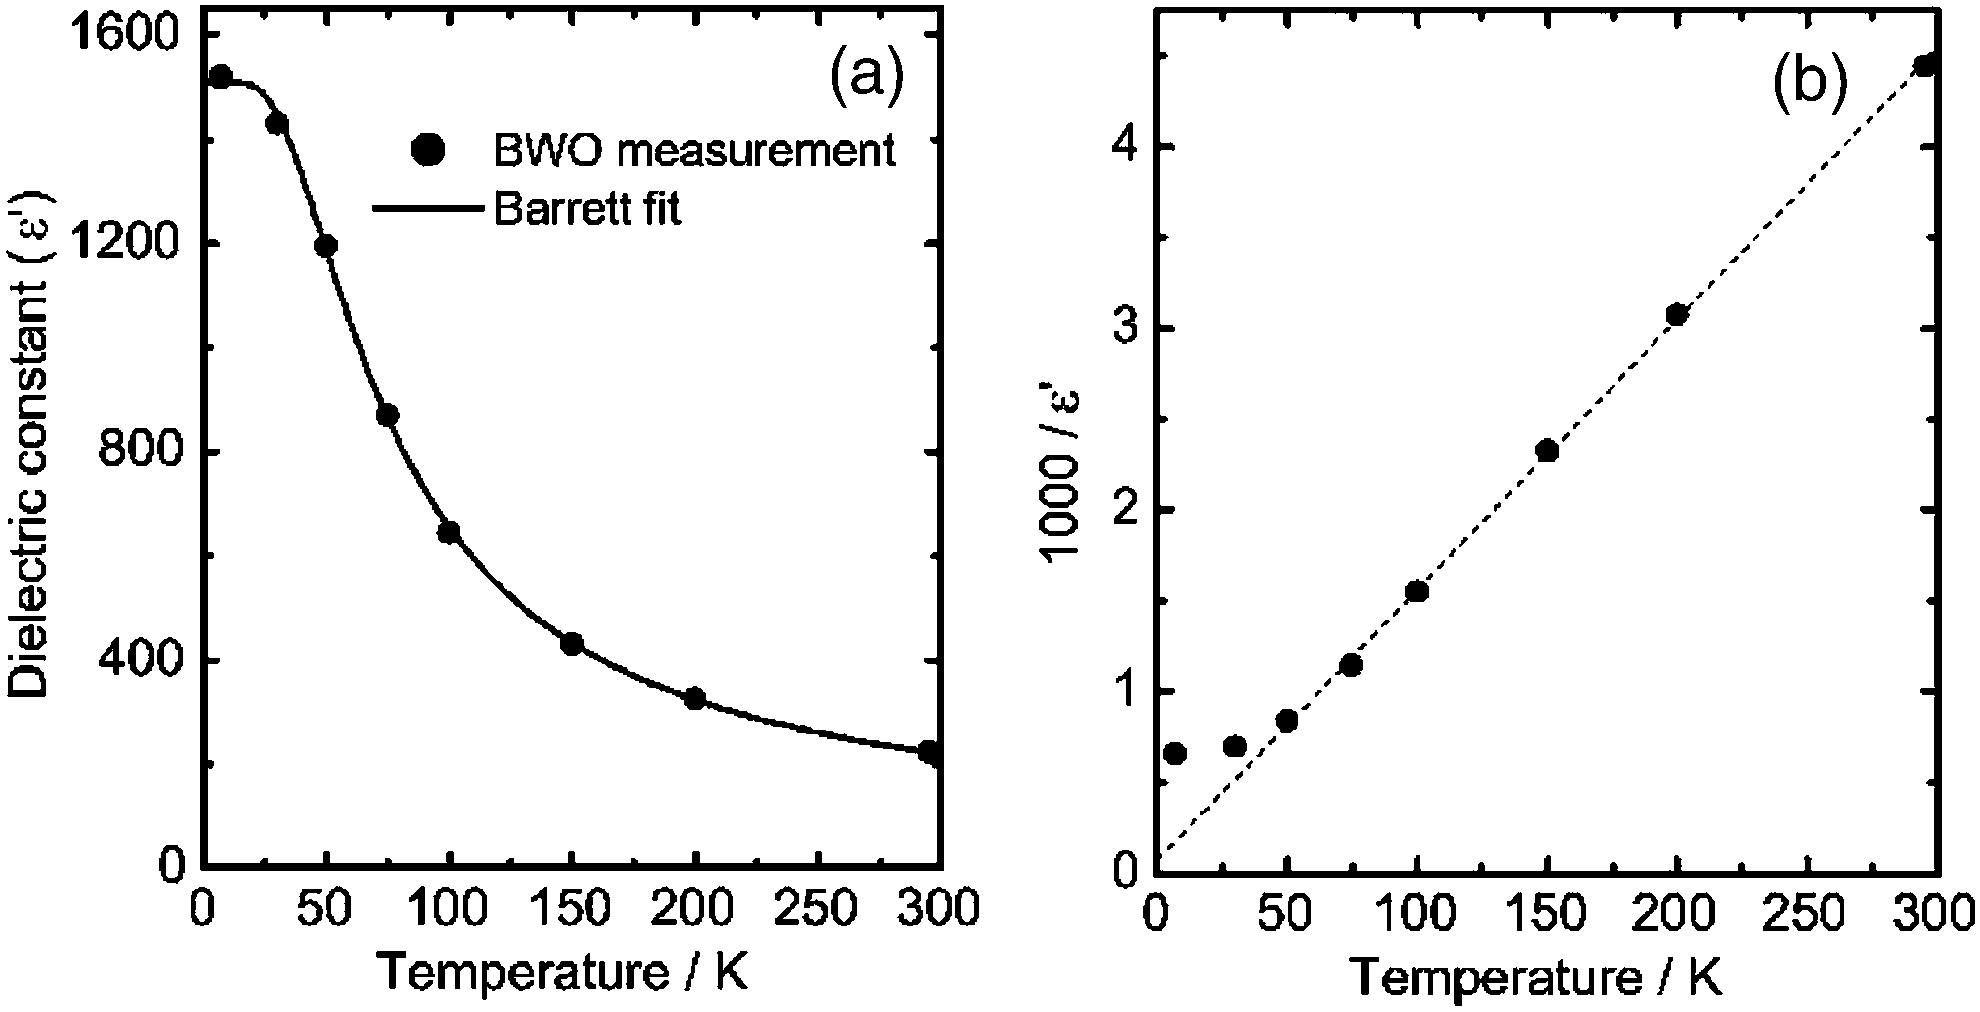
\includegraphics[width=\linewidth]{sto_barrett_curie_weiss.png}\par
      \vspace{0.02cm}
      {\fontsize{7.0}{8.2}\selectfont
        (a) mesures + Barrett : saturation de $\varepsilon'$ ;
        (b) tirets : Curie--Weiss classique.\par
        \textbf{Sous $50$ K, les données quittent la droite classique.}}
    \column{0.40\textwidth}
      \centering
      \tagline{Teal}{Interprétation microscopique}\par
      \vspace{0.04cm}
      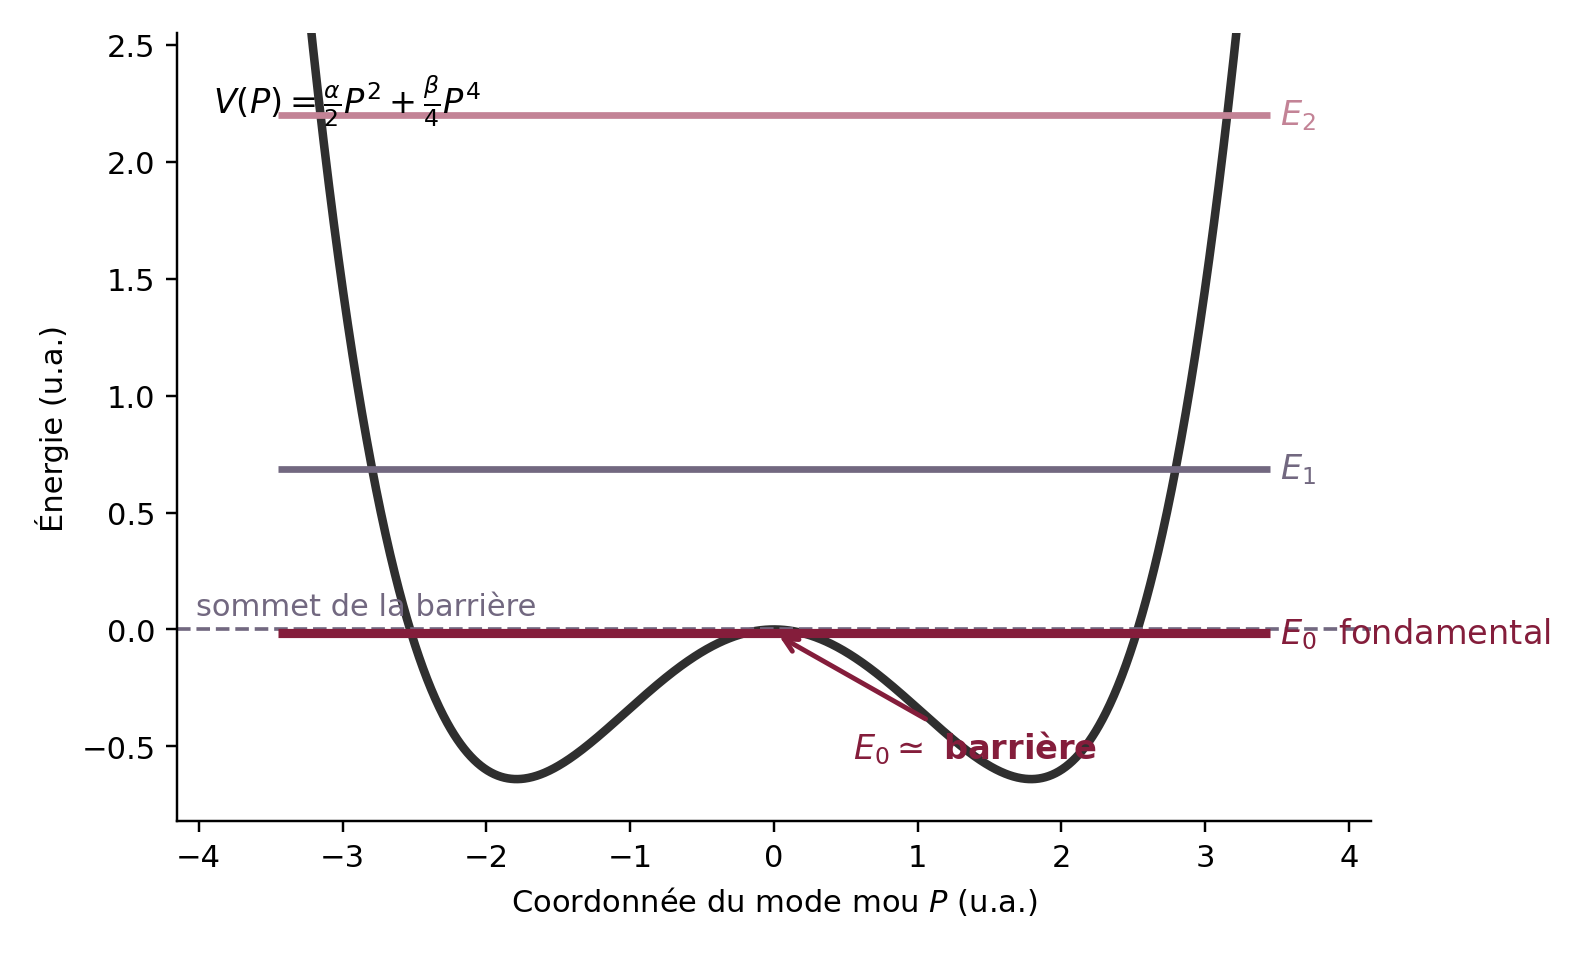
\includegraphics[height=2.82cm,keepaspectratio]{double_puit_niveaux.png}\par
      \vspace{0.03cm}
      {\small $E_0$ atteint presque la barrière :\par
      l'état reste délocalisé à $T=0$.}
  \end{columns}
  \vspace{0.12cm}
  {\centering\color{DeepNavy}\bfseries
  Les fluctuations de point zéro empêchent la localisation et saturent la susceptibilité.\par}
  \vspace{-0.08cm}
  \source{Fig. 14 : Balaya et al., \textit{J. Am. Ceram. Soc.} 89, 2804 (2006) ; Müller--Burkard (1979) ; spectre calculé pendant le stage.}
\end{frame}

\begin{frame}{Le mode mou ionique domine la réponse diélectrique}
  \begin{columns}[c,onlytextwidth]
    \column{0.43\textwidth}
      \centering
      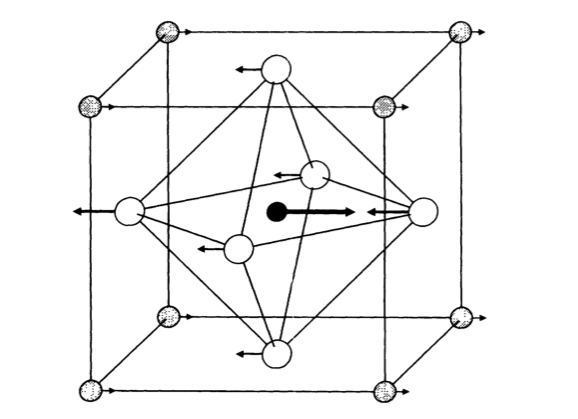
\includegraphics[width=0.76\linewidth]{mode_local.png}
      \source{Zhong, Vanderbilt et Rabe, \textit{Phys. Rev. Lett.} 73, 1861 (1994).}
    \column{0.53\textwidth}
      \begin{itemize}\setlength\itemsep{0.20cm}
        \item Chaque maille porte un vecteur $\bm u_i$ : le \textbf{déplacement collectif} associé au mode optique « mou ».
        \item Les déplacements de charges créent une polarisation locale :
        \[
          \bm P_i = \frac{Z^*}{\Omega_0}\,\bm u_i.
        \]
        \item Quand le mode devient très souple, un faible champ électrique produit une grande réponse.
      \end{itemize}
      \vspace{0.08cm}
      \begin{beamercolorbox}[rounded=true,sep=0.30em]{block body}
        \centering
        \begin{tikzpicture}[x=0.46cm,y=0.46cm,baseline=(current bounding box.center)]
          \draw[very thick,DeepNavy] (0.18,0.18) -- (0.18,1.62);
          \foreach \y in {0.28,0.58,...,1.48}
            \draw[Slate,line width=0.55pt] (0.18,\y) -- (-0.08,\y-0.18);
          \draw[decorate,decoration={coil,aspect=0.45,segment length=2.1mm,amplitude=1.7mm},
            line width=1.05pt,Teal] (0.18,0.90) -- (2.75,0.90);
          \node[font=\fontsize{6.5}{7.4}\selectfont\bfseries,text=Teal]
            at (1.45,1.45) {$k_{\rm eff}$};
          \draw[rounded corners=1.5pt,fill=PaleOrange,draw=CSOrange,line width=0.9pt]
            (2.75,0.42) rectangle (3.65,1.38);
          \node[font=\fontsize{7.0}{8.0}\selectfont\bfseries,text=CSOrange]
            at (3.20,0.90) {$u_i$};
          \draw[-{Latex[length=2.0mm]},very thick,PressureBlue]
            (3.68,0.90) -- (4.65,0.90);
          \node[font=\fontsize{6.5}{7.4}\selectfont\bfseries,text=PressureBlue]
            at (4.18,1.28) {$E$};
        \end{tikzpicture}
        \hspace{0.12cm}
        \begin{minipage}[c]{3.15cm}
          {\color{DeepNavy}\bfseries\fontsize{8.0}{9.3}\selectfont
            Ressort mou :
            $k_{\rm eff}\!\downarrow\Rightarrow u_i\!\uparrow\Rightarrow\chi\!\uparrow$.}
        \end{minipage}
      \end{beamercolorbox}
  \end{columns}
\end{frame}

% =============================================================================
% DEMARCHE SCIENTIFIQUE
% =============================================================================

\section{Modèle et méthode de calcul}

\begin{frame}{Le Hamiltonien effectif s'enrichit par ajouts successifs}
  \centering
  \begin{tikzpicture}[x=1cm,y=1cm,
    addbox/.style={rounded corners=2pt,minimum height=1.86cm,align=center,
      draw=Slate!45,line width=0.55pt,font=\small,text=DeepNavy}
  ]
    \draw[-{Latex[length=2.5mm]},thick,Slate] (0.18,2.46) -- (12.45,2.46);
    \node[font=\scriptsize\bfseries,text=Slate,fill=white,inner sep=2pt]
      at (6.31,2.46) {description enrichie pas à pas};

    \node[addbox,minimum width=2.62cm,fill=PaleOrange,draw=CSOrange]
      (polar) at (1.50,1.20) {%
        {\color{bordeauCS}\bfseries 1. Mode polaire}\\
        {\color{CSOrange}$H_{\rm local}+H_{\rm SR}+H_{\rm dip}$}\\
        {\scriptsize $\bm u_i$ : anharmonicité,}\\
        {\scriptsize courte portée et dipôles}};

    \node[addbox,minimum width=2.48cm,fill=HomStrainPurple!9!white,draw=HomStrainPurple]
      (hom) at (4.54,1.20) {%
        {\color{HomStrainPurple}\bfseries 2. Strain homogène}\\
        {\color{HomStrainPurple}$H_{\rm elas}^{\rm hom}(\bm\eta)$}\\
        {\scriptsize forme et volume}\\
        {\scriptsize globaux}};

    \node[addbox,minimum width=2.82cm,fill=InhomStrainGreen!9!white,draw=InhomStrainGreen]
      (inh) at (7.81,1.20) {%
        {\color{InhomStrainGreen}\bfseries 3. Strain inhomogène}\\
        {\color{InhomStrainGreen}$H_{\rm elas}^{\rm inh}(\{\bm w_i\})$}\\
        {\scriptsize $\bm w_i$ : modes acoustiques}\\
        {\scriptsize locaux}};

    \node[addbox,minimum width=2.32cm,fill=PressureBlue!8,draw=PressureBlue]
      (pressure) at (11.00,1.20) {%
        {\color{PressureBlue}\bfseries 4. Pression}\\
        {\color{PressureBlue}$p\Omega$}\\
        {\scriptsize contrainte hydrostatique}\\
        {\scriptsize externe}};
  \end{tikzpicture}

  \vspace{0.04cm}
  \begin{beamercolorbox}[rounded=true,sep=0.20em]{block body}
    \centering
    {\fontsize{6.5}{7.7}\selectfont
    \(\displaystyle
      \begin{aligned}
      H_{\mathrm{eff}}(p)={}&
      \sum_i\left(
        {\color{CSOrange}
          \frac{\bm\pi_{u,i}^{\,2}}{2M^*}
          +\frac12\alpha_0|\bm u_i|^2
          +\frac14\beta_{\alpha\beta\gamma\delta}
            u_i^\alpha u_i^\beta u_i^\gamma u_i^\delta
          +\frac16\gamma_{\alpha\beta\gamma\cdots\zeta}
            u_i^\alpha\cdots u_i^\zeta
          +\frac18\rho_{\alpha\beta\gamma\cdots\lambda}
            u_i^\alpha\cdots u_i^\lambda}
      \right)\\[-0.04cm]
      &+{\color{CSOrange}\frac12\sum_{i\ne j}u_i^\alpha
        \bigl(D_{ij}^{\alpha\beta}+J_{ij}^{\alpha\beta}\bigr)u_j^\beta}
      +{\color{HomStrainPurple}\frac{N}{2}\eta_\ell^{\mathrm{hom}}\mathcal B_{\ell m}
        \eta_m^{\mathrm{hom}}}\\[-0.04cm]
      &+{\color{InhomStrainGreen}\sum_i\frac{\bm\pi_{w,i}^{\,2}}{2M_w}}
      +{\color{InhomStrainGreen}\frac12\sum_{i,j}w_i^\alpha
        \Phi_{ij,\alpha\beta}^{\mathrm{elas,inh}}w_j^\beta}
      +\frac12\sum_{i,\ell,\alpha,\beta}B_{\ell\alpha\beta}
        \Bigl[{\color{HomStrainPurple}\eta_\ell^{\mathrm{hom}}}
        +{\color{InhomStrainGreen}\eta_{i,\ell}^{\mathrm{inh}}(\bm w)}\Bigr]
        u_i^\alpha u_i^\beta
      +\textcolor{PressureBlue}{p\Omega},
      \end{aligned}
    \)
    }
  \end{beamercolorbox}
  \source{Hamiltoniens effectifs de Zhong--Vanderbilt--Rabe (1995) et Nishimatsu et al. (2008, 2010, 2016).}
\end{frame}

\begin{frame}{Passer au continu change l'échelle, pas l'observable}
  \begin{columns}[T,onlytextwidth]
    \column{0.50\textwidth}
      \begin{beamercolorbox}[rounded=true,sep=0.40em]{block body}
        \centering
        {\bfseries\color{DeepNavy}Trois règles de passage}\par
        \vspace{0.05cm}
        \[
          \begin{aligned}
          \sum_i &\longrightarrow \int\!\frac{\mathrm d^3r}{\Omega_0},\\[0.16cm]
          \bm P(\bm r)&=\frac{Z^*}{\Omega_0}\,\bm u(\bm r),\\[0.16cm]
          \sum_{\bm k}&\longrightarrow
          \frac{\Omega}{(2\pi)^3}\int_{\mathrm{BZ}}\!\mathrm d^3k.
          \end{aligned}
        \]
      \end{beamercolorbox}
    \column{0.46\textwidth}
      \tagline{Teal}{Ce que l'on conserve}\par
      \begin{itemize}\setlength\itemsep{0.15cm}
        \item l'énergie totale ;
        \item la normalisation de la polarisation ;
        \item la coupure microscopique : la zone de Brillouin.
      \end{itemize}
      \vspace{0.14cm}
      \tagline{CSOrange}{Ce que l'on accepte de perdre}\par
      \begin{itemize}\setlength\itemsep{0.15cm}
        \item une interpolation réelle unique entre les mailles ;
        \item les variations plus fines que l'échelle du réseau.
      \end{itemize}
  \end{columns}
  \vspace{0cm}
  {\color{DeepNavy}\bfseries Le calcul est mené sur les modes de Fourier : aucune interpolation arbitraire n'est nécessaire.}
\end{frame}

\begin{frame}{Température finie : le temps imaginaire est un cercle}
  \begin{columns}[c,onlytextwidth]
    \column{0.43\textwidth}
      \tagline{CSOrange}{Intégrale de chemin de Feynman}\par
      \begin{beamercolorbox}[rounded=true,sep=0.28em]{block body}
        \centering
        {\fontsize{8.3}{9.9}\selectfont
        \(\displaystyle
          K(q_f,t_f;q_i,t_i)
          =\textcolor{CSOrange}{\langle q_f|e^{-i\hat H\Delta t/\hbar}|q_i\rangle}
        \)\par
        \vspace{0.10cm}
        \(\displaystyle
          =\int_{q_i}^{q_f}\!\mathcal Dq\;
          \textcolor{CSOrange}{e^{iS[q]/\hbar}} .
        \)}
      \end{beamercolorbox}
    \column{0.10\textwidth}
      \centering
      {\color{Teal}\bfseries $t=-i\tau$}\par
      \vspace{0.08cm}
      {\color{Teal}\Large$\Longrightarrow$}
    \column{0.43\textwidth}
      \tagline{Teal}{Intégrale fonctionnelle de champ}\par
      \begin{beamercolorbox}[rounded=true,sep=0.28em]{block body}
        \centering
        {\fontsize{8.3}{9.9}\selectfont
        \(\displaystyle
          Z(\beta)=\operatorname{Tr}e^{-\beta\hat H}
          =\sum_a e^{-\beta E_a}
        \)\par
        \vspace{0.05cm}
        {\fontsize{7.1}{8.4}\selectfont
        \(\displaystyle
          =\int\!\mathcal D\phi\;
          \textcolor{Teal}{\langle\phi(\bm r)|e^{-\beta\hat H}|\phi(\bm r)\rangle}
        \)\par}
        \vspace{0.05cm}
        \(\displaystyle
          =\oint_{\phi(\beta\hbar)=\phi(0)}\!\mathcal D\phi\;
          \textcolor{Teal}{e^{-S_E[\phi]/\hbar}} .
        \)}
      \end{beamercolorbox}
  \end{columns}

  \vspace{0.11cm}
  \tagline{WarmGold}{La périodicité discrétise les fréquences}\par
  \vspace{0.03cm}
  \begin{beamercolorbox}[rounded=true,sep=0.22em]{block body}
    \begin{columns}[c,onlytextwidth]
      \column{0.25\textwidth}
        \centering
        {\color{Teal}\fontsize{22}{22}\selectfont $\bigcirc$\par}
        \vspace{-0.04cm}
        {\fontsize{6.9}{8.0}\selectfont
          cercle : $\tau\sim\tau+\beta\hbar$}
      \column{0.19\textwidth}
        \centering
        {\color{DeepNavy}\fontsize{8.2}{9.5}\selectfont
          $\xrightarrow{\ \mathrm{TF}\ \text{en }\tau\ }$}
      \column{0.50\textwidth}
        \centering
        {\color{DeepNavy}\bfseries\fontsize{7.7}{9.0}\selectfont
          Fréquences de Matsubara discrètes\par}
        \vspace{0.02cm}
        {\fontsize{8.1}{9.4}\selectfont
          $\displaystyle \omega_n=\frac{2\pi n}{\beta\hbar}
          =\frac{2\pi n k_BT}{\hbar},\quad n\in\mathbb Z$}
    \end{columns}
  \end{beamercolorbox}
  \vspace{-0.24cm}
  \source{E. C. Marino, \textit{Quantum Field Theory Approach to Condensed Matter Physics}, Cambridge University Press (2017).}
\end{frame}

% Slide 14 mise en réserve temporairement.
\iffalse
\begin{frame}{Le temps imaginaire unifie le thermique et le quantique}
  \begin{columns}[c,onlytextwidth]
    \column{0.48\textwidth}
      \centering
      \begin{tikzpicture}[x=0.75cm,y=0.75cm]
        \draw[very thick,DeepNavy] (0,0) circle (2.15);
        \foreach \a/\lab in {90/$0$,30/$\tau$, -90/$\beta\hbar$,210/$$}{
          \fill[CSOrange] (\a:2.15) circle (2.1pt);
          \node[Slate] at (\a:2.55) {\lab};
        }
        \draw[-{Latex[length=2.5mm]},very thick,Teal] (100:2.38) arc[start angle=100,end angle=-190,radius=2.38];
        \node[align=center,text=DeepNavy] at (0,0) {temps imaginaire\\\bfseries périodique};
        \node[align=center,text=Slate] at (0,-3.75) {$\omega_n=\dfrac{2\pi n k_BT}{\hbar}$};
      \end{tikzpicture}
    \column{0.48\textwidth}
      \begin{itemize}\setlength\itemsep{0.24cm}
        \item La fonction de partition quantique devient une intégrale sur $\bm P(\bm r,\tau)$.
        \item La périodicité impose des fréquences discrètes de Matsubara.
        \item Après sommation, chaque mode contribue par
        \[
          \langle\delta P^2\rangle_{\omega}
          \propto \frac{1}{2m\omega}
          \coth\!\left(\frac{\hbar\omega}{2k_BT}\right).
        \]
      \end{itemize}
      \takeaway{Entrée de la SCHA : cette covariance réunit agitation thermique et mouvement de point zéro.}
  \end{columns}
\end{frame}
\fi

{
\setbeamerfont{frametitle}{series=\bfseries,size=\fontsize{16.5}{19}}
\begin{frame}[label=slide13-closed]{L'anharmonicité génère la boucle qui corrige la rigidité}
  \begin{columns}[T,onlytextwidth]
    \column{0.43\textwidth}
      \tagline{CSOrange}{Théorie libre : forme quadratique}\par
      \vspace{0.03cm}
      \begin{beamercolorbox}[rounded=true,sep=0.20em]{block body}
        \centering
        {\fontsize{7.9}{9.4}\selectfont
        \(\displaystyle
          \mathcal L_0=
          -\frac12\,\phi\,(\Box+m^2)\,\phi
        \)\par
        \vspace{0.06cm}
        \(\displaystyle
          S_0=\frac12\int\!\mathrm d^4x\,\mathrm d^4y\;
          \phi(x)\,G^{-1}(x-y)\,\phi(y)
        \)}
      \end{beamercolorbox}

    \column{0.10\textwidth}
      \vspace{0.72cm}
      \centering
      \makebox[0pt][c]{%
        {\bfseries\fontsize{7.5}{9.0}\selectfont
        \(\begin{gathered}
          \textcolor{CSOrange}{\phi}\equiv\textcolor{Teal}{\bm x}\\[0.10cm]
          \textcolor{CSOrange}{G}\equiv\textcolor{Teal}{\bm A^{-1}}\\[0.10cm]
          \textcolor{Teal}{N}\longrightarrow\textcolor{CSOrange}{\infty}
        \end{gathered}\)}%
      }

    \column{0.43\textwidth}
      \tagline{Teal}{Gaussienne en $N$D}\par
      \vspace{0.03cm}
      \begin{beamercolorbox}[rounded=true,sep=0.20em]{block body}
        \centering
        {\fontsize{7.2}{8.6}\selectfont
        \(\displaystyle
          \int_{\mathbb R^N}\!\mathrm d^N x\,
          e^{-\frac12\bm x^{\mathsf T}\bm A\bm x
             +\bm J^{\mathsf T}\bm x}
        \)\par
        \vspace{0.14cm}
        {\color{bordeauCS}\fontsize{6.65}{7.45}\selectfont
          \(\int_{\mathbb R}\!\mathrm dx\,e^{-\alpha x^2- \lambda x^4} =\ ?\)\par
          \vspace{-0.01cm}\textbf{pas de formule simple}}
        }
      \end{beamercolorbox}
  \end{columns}

  \vspace{-0.04cm}
  {\fontsize{8.6}{10.1}\selectfont
  \tagline{Teal}{L'interaction développe autour de cette gaussienne}\par}
  \vspace{0.02cm}
  {\centering\fontsize{7.2}{8.6}\selectfont
    \(\displaystyle
      \mathcal L_{\mathrm{int}}=-\frac{\lambda}{4!}\phi^4,
      \qquad
      e^{iS_{\mathrm{int}}}
      =\sum_{n=0}^{\infty}\frac{1}{n!}
      \left[-\frac{i\lambda}{4!}
      \int\!\mathrm d^4z\,\phi^4(z)\right]^n,
      \qquad
      \langle\phi\phi\rangle\overset{?}{=}G+\mathcal O(\lambda).
    \)\par}

  \vspace{-0.02cm}
  {\fontsize{9.8}{11.4}\selectfont
  \tagline{CSOrange}{Premier ordre : la contraction tadpole}\par}
  \vspace{0.04cm}
  \begin{columns}[c,onlytextwidth]
    \column{0.70\textwidth}
      {\fontsize{8.2}{9.8}\selectfont
      \(\displaystyle
        \frac{\lambda}{4!}
        \langle0|T\phi(x)\phi(y)\phi^4(z)|0\rangle_{0,c}
        =\frac{\lambda}{2}\,
        G(x-z)\,G(0)\,G(z-y).
      \)}
      \vspace{0.08cm}

      {\fontsize{7.6}{8.9}\selectfont\bfseries\color{CSOrange}
      Mode mou : fluctuations fortes à tout ordre $\Longrightarrow$ troncature perturbative fragile.}
    \column{0.26\textwidth}
      \centering
      {\color{Teal}\bfseries\fontsize{8.4}{9.6}\selectfont
      $\Longleftrightarrow$\par}
      \vspace{0.03cm}
      \begin{tikzpicture}[x=0.46cm,y=0.46cm,
        prop/.style={draw=DeepNavy,line width=1.05pt},
        vertex/.style={fill=CSOrange,draw=CSOrange,circle,inner sep=1.4pt}]
        \draw[prop] (0,0) -- (3.8,0);
        \node[vertex] at (1.9,0) {};
        \draw[prop] (1.9,0.56) circle (0.56);
        \node[font=\fontsize{6.5}{7.2}\selectfont,text=Slate]
          at (0.20,-0.34) {$x$};
        \node[font=\fontsize{6.5}{7.2}\selectfont,text=Slate]
          at (1.9,-0.34) {$z$};
        \node[font=\fontsize{6.5}{7.2}\selectfont,text=Slate]
          at (3.60,-0.34) {$y$};
        \node[font=\fontsize{6.5}{7.2}\selectfont\bfseries,text=Teal]
          at (1.9,1.50) {$G(0)$};
      \end{tikzpicture}
  \end{columns}

  \begin{tikzpicture}[remember picture,overlay]
    \node[anchor=east] at
      ([xshift=-0.55cm,yshift=-5.25cm]current page.north east) {%
      \hyperlink{slide13-popup}{\beamergotobutton{Hamiltonien complet}}};
  \end{tikzpicture}
  \vspace{-0.17cm}
\end{frame}
}

\begin{frame}[label=qa-scha]{\hspace*{0.22cm}La SCHA choisit un ressort renormalisé}
  \centering
  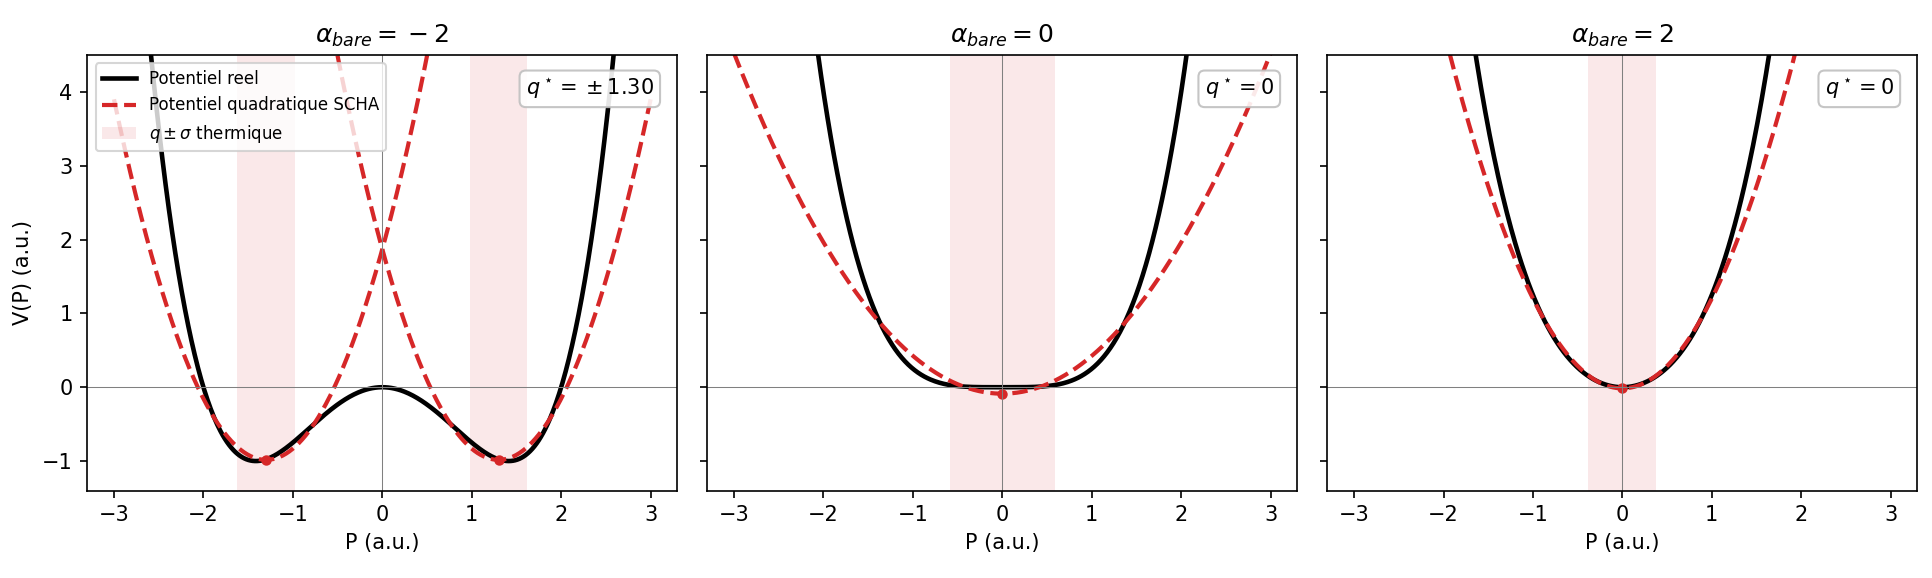
\includegraphics[width=0.86\linewidth]{double_puit_scha.png}
  \vspace{0.08cm}
  \begin{columns}[T,onlytextwidth]
    \column{0.31\textwidth}
      \tagline{CSOrange}{1. Essai}\par
      Choisir un potentiel quadratique de rigidité $A(T)$.
    \column{0.31\textwidth}
      \tagline{Teal}{2. Évaluation}\par
      Calculer ses fluctuations thermiques et quantiques.
    \column{0.31\textwidth}
      \tagline{WarmGold}{3. Auto-cohérence}\par
      Ajuster $A(T)$ jusqu'à reproduire les fluctuations du potentiel réel.
  \end{columns}
  \vspace{0.06cm}
  {\fontsize{8.0}{9.3}\selectfont\bfseries\color{DeepNavy}
  $A(T)$ dépend ainsi de ses propres fluctuations, sans troncature à ordre fixe.\par}
  \vspace{-0.10cm}
  \source{figure produite pendant le stage ; principe variationnel de Gibbs--Bogoliubov / SCHA.}
\end{frame}

\begin{frame}{L'auto-cohérence resomme les diagrammes de Hartree}
  \begin{columns}[T,onlytextwidth]
    \column{0.56\textwidth}
      \tagline{CSOrange}{Équation résolue numériquement}\par
      \vspace{0.04cm}
      \begin{beamercolorbox}[rounded=true,sep=0.40em]{block body}
        \[
          \boxed{
          \begin{aligned}
          A_1={}&A_{0,1}+\mathcal P^{(p)}\\[-1pt]
          &+\Delta A_1^{\mathrm{SCHA}}
          \big[\bar{\bm G}(A_1;T)\big]
          \end{aligned}}
        \]
      \end{beamercolorbox}

      \vspace{0.16cm}
      \tagline{Teal}{La boucle dépend elle-même de $A_1$}\par
      \vspace{0.02cm}
      \[
        \bar G_{ab}(A_1;T)
        =\frac{\Omega_0}{\beta(2\pi)^3}
        \!\int_{\mathrm{BZ}}\!\mathrm d^3k
        \sum_n
        \big[A_{\rm trial}(\bm k,\omega_n)^{-1}\big]_{ab}.
      \]
    \column{0.40\textwidth}
      \centering
      \tagline{WarmGold}{Diagrammes de Feynman}\par
      \vspace{0.08cm}
      \[
        A=A_0+\Sigma_{\mathrm H}[G],\qquad G=A^{-1}
      \]
      \vspace{-0.08cm}
      \begin{tikzpicture}[x=0.59cm,y=0.60cm,
        bare/.style={draw=DeepNavy,line width=1.0pt},
        loop/.style={draw=DeepNavy,line width=1.0pt},
        vertex/.style={fill=CSOrange,draw=CSOrange,circle,inner sep=1.4pt}
      ]
        % Le propagateur est égal à la série de Dyson--Hartree.
        \draw[bare] (0.0,1.45) -- (0.95,1.45);
        \node[font=\scriptsize,above] at (0.48,1.50) {$G$};
        \node[font=\bfseries] at (1.25,1.45) {$=$};

        \draw[bare] (1.55,1.45) -- (2.50,1.45);
        \node[font=\scriptsize,below] at (2.03,1.40) {$G_0$};
        \node[font=\bfseries] at (2.78,1.45) {$+$};

        \draw[bare] (3.05,1.45) -- (4.35,1.45);
        \node[vertex] at (3.70,1.45) {};
        \draw[loop] (3.70,1.94) circle (0.49);
        \node[font=\scriptsize,text=Teal,align=center] at (3.70,2.88)
          {boucle\ $G$};
        \node[font=\bfseries] at (4.64,1.45) {$+$};

        \draw[bare] (4.95,1.45) -- (6.85,1.45);
        \node[vertex] at (5.42,1.45) {};
        \node[vertex] at (6.38,1.45) {};
        \draw[loop] (5.42,1.83) circle (0.38);
        \draw[loop] (6.38,1.83) circle (0.38);
        \node[font=\bfseries\large] at (7.20,1.45) {$\cdots$};

        \draw[-{Latex[length=2.1mm]},thick,Teal]
          (6.35,2.62) .. controls (5.85,3.30) and (1.45,3.30) .. (0.55,2.05);
        \node[font=\scriptsize\bfseries,text=Teal,fill=white,inner sep=1pt]
          at (3.55,3.20) {auto-cohérence};

        \node[align=center,font=\small\bfseries,text=DeepNavy]
          at (3.55,0.35) {0, 1, 2, $\ldots$ boucles de Hartree\\
          « daisy / superdaisy »};
      \end{tikzpicture}
  \end{columns}

  \vspace{0.16cm}
  {\centering\bfseries\color{DeepNavy}
  Pourquoi ce choix ? Une racine resomme cette classe infinie --- pas la série complète.\par}
  \source{solveur SCHA du stage ; Xiao--Marianetti, \textit{PRB} 107, 094303 (2023).}
\end{frame}

{
\setbeamerfont{frametitle}{series=\bfseries,size=\fontsize{15.5}{18}}
\begin{frame}{Chaîne numérique et auto-détermination de la rigidité/masse}
  \begin{columns}[c,onlytextwidth]
    \column{0.48\textwidth}
      \centering
      \begin{tikzpicture}[
        box/.style={rounded corners=2pt,minimum width=3.45cm,minimum height=0.74cm,align=center,font=\bfseries},
        flow/.style={-{Latex[length=2.5mm]},very thick,Slate}
      ]
        \node[box,fill=PaleOrange,text=DeepNavy] (a) {rigidité test $A_1$};
        \node[box,fill=Mist,text=DeepNavy,below=0.35cm of a] (m) {fréquences des modes $\omega_i(\bm k)$};
        \node[box,fill=PaleTeal,text=DeepNavy,below=0.35cm of m] (g) {fluctuations $\bar G[A_1;T]$};
        \node[box,fill=PaleGold,text=DeepNavy,below=0.35cm of g] (c) {corrections anharmoniques $\Delta A_1$};
        \draw[flow] (a) -- (m);
        \draw[flow] (m) -- (g);
        \draw[flow] (g) -- (c);
        \draw[flow] (c.east) -- ++(0.60,0) |- (a.east);
      \end{tikzpicture}
    \column{0.48\textwidth}
      \begin{beamercolorbox}[rounded=true,sep=0.42em]{block body}
        \[
          \begin{aligned}
          A_1={}&A_{0,1}+\mathcal P^{(p)}
          +\Delta A^{(4)}_{\rm loc}
          +\Delta A^{(4)}_{\rm hom}\\
          &+\Delta A^{(4)}_{\rm inh}
          +\Delta A^{(6)}+\Delta A^{(8)}.
          \end{aligned}
        \]
      \end{beamercolorbox}
      \vspace{0.14cm}
      Une fois la racine stable trouvée :
      \[
        \boxed{\bm\chi_{\rm stat}(T)=\Omega_0\,\bm A^{-1}(\bm 0,0;T)}
      \]
      \vspace{0.04cm}
      {\color{DeepNavy}\bfseries La réponse gaussienne est l'inverse du ressort renormalisé.}
  \end{columns}

  \vspace{0.18cm}
  \centering
  \begin{tikzpicture}[
    node distance=0.22cm,
    flowbox/.style={rounded corners=2pt,minimum width=2.08cm,minimum height=1.06cm,align=center,font=\small\bfseries},
    arr/.style={-{Latex[length=2.1mm]},thick,Slate}
  ]
    \node[flowbox,fill=PaleOrange,text=DeepNavy] (p) {paramètres\\publiés};
    \node[flowbox,fill=Mist,text=DeepNavy,right=of p] (k) {noyaux\\périodiques};
    \node[flowbox,fill=PaleTeal,text=DeepNavy,right=of k] (q) {quadrature\\$\bm k$};
    \node[flowbox,fill=PaleGold,text=DeepNavy,right=of q] (d) {diagonalisation\\$3\times3$};
    \node[flowbox,fill=Mist,text=DeepNavy,right=of d] (r) {racine\\auto-cohérente};
    \node[flowbox,fill=PaleOrange,text=DeepNavy,right=of r] (x) {$\chi(T)$\\et diagnostics};
    \draw[arr] (p)--(k); \draw[arr] (k)--(q); \draw[arr] (q)--(d);
    \draw[arr] (d)--(r); \draw[arr] (r)--(x);
  \end{tikzpicture}
  \source{solveurs Python développés pendant le stage ; quadrature de Gauss--Legendre et recherche de racine par encadrement.}
\end{frame}
}

% Slide 18 mise en réserve temporairement.
\iffalse
\begin{frame}{Quatre difficultés ont structuré le travail d'ingénierie}
  \fontsize{8.6}{10.0}\selectfont
  \begin{tabularx}{\linewidth}{@{}>{\RaggedRight\arraybackslash\bfseries\color{DeepNavy}}p{0.25\linewidth} X >{\RaggedRight\arraybackslash}p{0.25\linewidth}@{}}
    \toprule
    Difficulté & Décision mise en œuvre & Preuve / garde-fou \\
    \midrule
    Somme dipolaire conditionnelle & Décomposition d'Ewald réelle + réciproque & Convention et terme de contact explicités \\
    \addlinespace[0.08cm]
    Développement $k^2$ instable au bord de zone & Noyau périodique complet à 26 voisins dans les intégrales & Aucun mode non physique au point $R$ \\
    \addlinespace[0.08cm]
    Plusieurs racines auto-cohérentes & Encadrement, sélection de branche et contrôle $\mu_{\min}>0$ & Échecs conservés comme tels, pas interpolés \\
    \addlinespace[0.08cm]
    Variables singulières quand $T\to0$ & Résolution en déplacement $\bm u_{\min}$ et covariance physique $\bar{\bm G}$ & Point $T=0$ calculé directement \\
    \bottomrule
  \end{tabularx}
  \vspace{0.16cm}
  {\color{DeepNavy}\bfseries Apport clé : des conditions de validité testables, pas seulement une formule.}
\end{frame}
\fi

\begin{frame}[shrink=2]{\fontsize{17.5}{20}\selectfont Exemple de difficultés techniques : le mode $\bm k=0$ garde la mémoire des surfaces}
  \begin{columns}[T,onlytextwidth]
    \column{0.52\textwidth}
      \centering
      \begin{tikzpicture}[
        x=0.86cm,y=0.86cm,
        pol/.style={-{Latex[length=2.0mm]},line width=1.1pt,bordeauCS}
      ]
        \node[font=\small\bfseries,text=DeepNavy] at (2.15,2.18)
          {Bulk en conditions périodiques};
        \foreach \i in {0,1,2}{
          \foreach \j in {0,1}{
            \filldraw[fill=Mist,draw=Slate!55]
              ({1.45*\i},{0.90*\j}) rectangle ++(1.34,0.80);
          }
        }
        \filldraw[fill=PaleOrange,draw=bordeauCS,very thick]
          (1.45,0.90) rectangle ++(1.34,0.80);
        \foreach \i in {0,1,2}{
          \foreach \j in {0,1}{
            \foreach \dy in {0.25,0.55}{
              \draw[pol]
                ({1.45*\i+0.25},{0.90*\j+\dy}) -- ++(0.82,0);
            }
          }
        }
        \node[font=\scriptsize,text=Slate] at (2.15,-0.26)
          {la maille centrale est recopiée : aucun bord explicite};

        \node[font=\small\bfseries,text=DeepNavy] at (2.15,-0.82)
          {Échantillon fini, $\bm P$ uniforme};
        \filldraw[fill=PaleTeal,draw=Slate,rounded corners=1pt]
          (0.18,-2.52) rectangle (4.12,-1.38);
        \foreach \dy in {-2.14,-1.82}{
          \draw[pol] (0.60,\dy) -- (1.68,\dy);
          \draw[pol] (2.62,\dy) -- (3.70,\dy);
        }
        \node[font=\scriptsize\bfseries,text=DeepNavy]
          at (2.15,-1.55) {$\bm P$};
        \node[font=\scriptsize\bfseries,text=Teal]
          at (2.15,-2.38) {$\rho_{\text{liée}}=0$ dans le volume};
        \foreach \dy in {-2.32,-1.95,-1.58}{
          \node[font=\small\bfseries,text=bordeauCS] at (0.02,\dy) {$-$};
          \node[font=\small\bfseries,text=bordeauCS] at (4.28,\dy) {$+$};
        }
        \node[font=\scriptsize,text=Slate,anchor=north east]
          at (0.22,-2.64) {$\sigma_{\text{liée}}<0$};
        \node[font=\scriptsize,text=Slate,anchor=north west]
          at (4.08,-2.64) {$\sigma_{\text{liée}}>0$};
      \end{tikzpicture}

    \column{0.45\textwidth}
      \fontsize{8.6}{9.9}\selectfont
      \tagline{CSOrange}{Une convergence conditionnelle}

      {\scriptsize Ordre / forme de sommation $\Rightarrow$ valeur obtenue.}
      \vspace{-0.18cm}
      {\small
        \[
          E_{\rm dip}=E_{\text{réel}}+E_{\bm k\neq0}+E_{\rm self}
          +\textcolor{bordeauCS}{E_{\bm k=0}}.
        \]
      }
      \vspace{-0.26cm}

      \tagline{Teal}{Les charges liées}
      \vspace{-0.10cm}
      {\small
        \[
          \rho_{\text{liée}}=-\bm\nabla\!\cdot\!\bm P,
          \qquad
          \sigma_{\text{liée}}=\bm P\!\cdot\!\bm n.
        \]
      }
      \vspace{-0.26cm}

      \tagline{WarmGold}{Le point $\bm k=0$ n'est pas fixé par le bulk}
      \vspace{0.12cm}
      {\centering\small
        $D^{\rm non\text{-}ana}_{\alpha\beta}(\bm k)
        \propto k_\alpha k_\beta/k^2$\par
        \vspace{0.04cm}
        {\scriptsize $\bm k\to0$ : la limite dépend de la direction.\par}}
      \vspace{0.14cm}
      {\centering\small
        $\boxed{E_{\bm k=0}\propto\bm P\!\cdot\!\bm N\bm P}$\par}
      \vspace{0.16cm}
      {\scriptsize\color{Slate}$\bm N$ : forme des bords ;
      métal (« tin foil ») $\Rightarrow E_{\bm k=0}=0$.}
  \end{columns}

  \vspace{-0.08cm}
  \source{Campbell (1963) ; Borwein et al. (1985) ; Nishimatsu et al., \textit{Phys. Rev. B} 82, 134106 (2010).}
\end{frame}

% =============================================================================
% RESULTATS
% =============================================================================

\section{Résultats et diagnostics}

\begin{frame}[label=qa-bto]{BaTiO$_3$ : corriger le volume ne corrige pas la réponse}
  \begin{columns}[c,onlytextwidth]
    \column{0.62\textwidth}
      \centering
      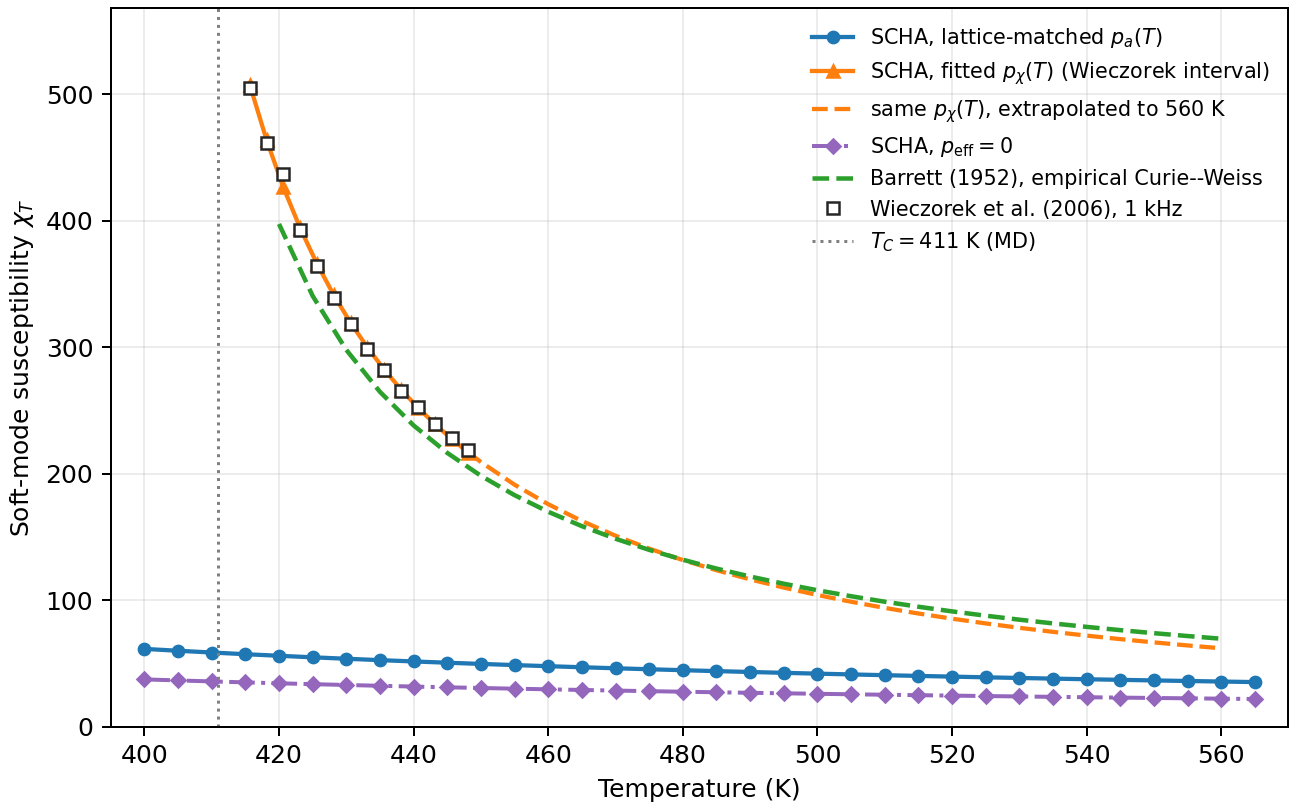
\includegraphics[width=0.94\linewidth]{chi_temperature_400_565K_inhomogeneous_quartic.png}
    \column{0.34\textwidth}
      {\fontsize{8.7}{10.2}\selectfont
      \begin{itemize}\setlength\itemsep{0.06cm}
        \item \textbf{Bleu :} $p_a(T)$ reproduit le paramètre de maille
        attendu, mais $\chi(T)$ reste sous-estimée.
        \item \textbf{Orange :} $p_\chi(T)$ minimise l'écart quadratique
        aux 14 points entre $415{,}65$ et $448{,}15$ K
        (tirets : extrapolation).
        \item \textbf{À $403\,\mathrm K$ :} $p_a(T)$ reproduit la
        référence de Nishimatsu, $a=4{,}010$ \AA\ juste au-dessus de
        $T_C$ ; la \textbf{maille équivalente à $403\,\mathrm K$} pour
        $p_\chi$ vaut $a_\chi\simeq4{,}043$ \AA.
      \end{itemize}
      \vspace{0.01cm}
      {\color{CSOrange}\bfseries Diagnostic :} contre-terme effectif,
      pas prédiction indépendante.\par
      \vspace{0.05cm}
      {\color{Teal}\bfseries\fontsize{13.5}{15.5}\selectfont 0,52\,\%}
      {\fontsize{7.8}{9.2}\selectfont erreur relative moyenne}}
  \end{columns}
  \vspace{-0.13cm}
  \source{calcul du stage ; $a(T)$ de Nakatani et al. (2016) ; données 1 kHz de Wieczorek et al. (2006) ; Barrett (1952).}
\end{frame}

\begin{frame}{L'écart devient un diagnostic du modèle}
  \begin{columns}[T,onlytextwidth]
    \column{0.47\textwidth}
      \begin{block}<1->{Ce que le modèle explique}
        \begin{itemize}\setlength\itemsep{0.11cm}
          \item la décroissance qualitative de $\chi(T)$ ;
          \item l'effet séparé des couplages local, homogène et acoustique ;
          \item la sensibilité extrême au volume et à la rigidité du mode mou.
        \end{itemize}
      \end{block}
    \column{0.49\textwidth}
      \begin{block}<2->{Ce que l'écart révèle}
        \begin{itemize}\setlength\itemsep{0.11cm}
          \item une correction hydrostatique ne remplace pas tous les phonons éliminés ;
          \item des modes optiques plus énergétiques peuvent renormaliser $T_C$ et $\chi$ séparément ;
          \item la fermeture gaussienne SCHA peut elle-même sous-estimer les fluctuations près de $T_C$.
        \end{itemize}
      \end{block}
  \end{columns}
  \vspace{0.08cm}
  \uncover<3->{%
    \begin{beamercolorbox}[rounded=true,sep=0.26em]{block body}
      {\color{WarmGold}\bfseries Cadre de validité.}\quad
      Modes optiques secondaires, rotation de SrTiO$_3$ et fluctuations critiques restent partiellement absents ;
      une branche stable n'est pas forcément le minimum global et les mesures dépendent de la microstructure.
    \end{beamercolorbox}
    \vspace{0.05cm}
    {\color{DeepNavy}\bfseries Décision : le fit mesure le « ramollissement manquant » ; il ne constitue pas une loi physique.}%
  }
  \vspace{-0.10cm}
  \source{interprétation cohérente avec Mayer et al., \textit{Phys. Rev. B} 106, 064108 (2022).}
\end{frame}

\begin{frame}[label=qa-missing]{Des modes optiques éliminés peuvent renormaliser $T_C$}
  \begin{columns}[T,onlytextwidth]
    \column{0.57\textwidth}
      \centering
      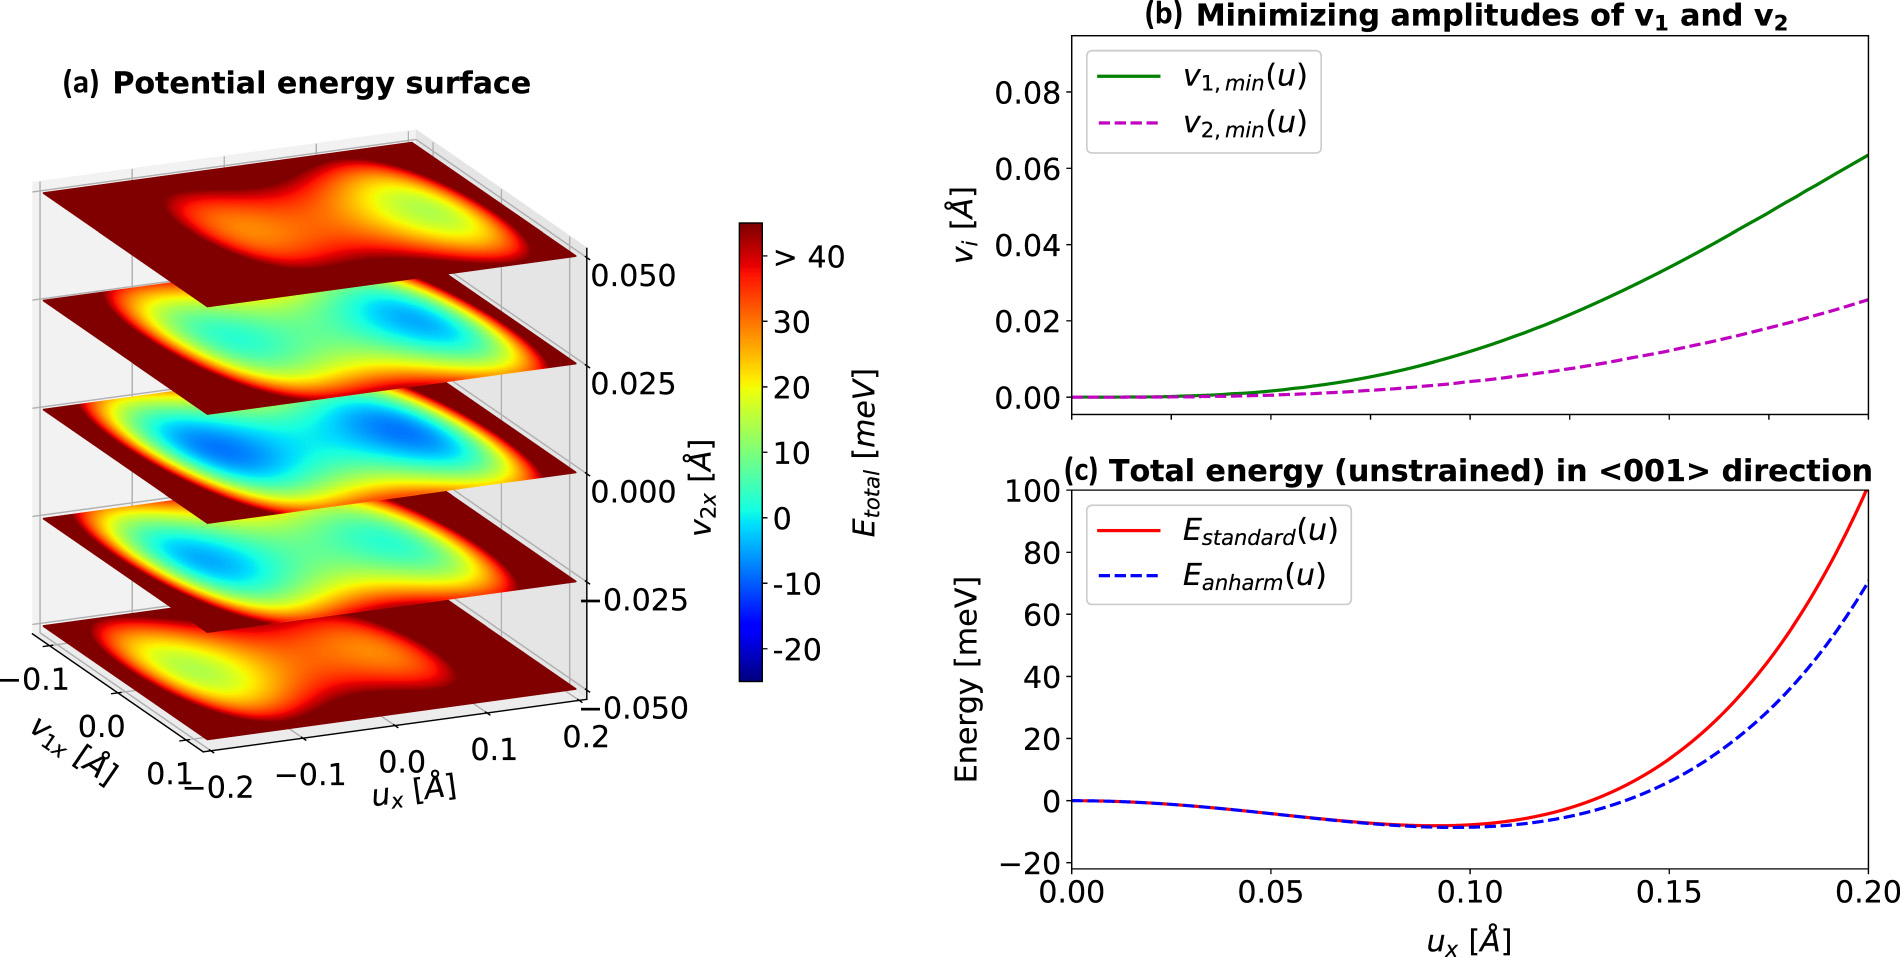
\includegraphics[width=0.98\linewidth]{mayer2022_anharmonic_coupling_fig1.png}
      \vspace{0.02cm}

      {\color{Slate}\fontsize{6.8}{7.8}\selectfont
      $E(u,v_1,v_2)$, amplitudes minimisantes, puis potentiel effectif
      $E_{\rm eff}(u)$.\par}
    \column{0.39\textwidth}
      \tagline{CSOrange}{Deux modes optiques $\Gamma_{15}$ manquants}\par
      \vspace{0.05cm}
      {\centering\fontsize{10.5}{12.5}\selectfont
      $v_1=178\,\mathrm{cm}^{-1}
      \qquad v_2=468\,\mathrm{cm}^{-1}$\par}

      \vspace{0.10cm}
      \tagline{Teal}{Couplages mixtes avec $u$}\par
      \vspace{0.05cm}
      {\centering\fontsize{9.5}{11.5}\selectfont
      $\Delta E_{\rm anh}\supset
      uv_i,\ u^3v_i,\ u^2v_i^2,\ uv_i^3,\ldots$\par}

      \vspace{0.10cm}
      \tagline{WarmGold}{Élimination adiabatique}\par
      \vspace{0.05cm}
      \begin{beamercolorbox}[rounded=true,sep=0.22em]{block body}
        \centering\fontsize{10}{12}\selectfont
        $\displaystyle
        E_{\rm eff}(u)=\min_{v_1,v_2}E(u,v_1,v_2)$
      \end{beamercolorbox}
      \vspace{0.05cm}
      {\fontsize{7.4}{8.6}\selectfont
      $v_1$ et $v_2$ sont minimisés, pas gardés comme modes dynamiques.}
  \end{columns}

  \vspace{0.05cm}
  \begin{beamercolorbox}[wd=\linewidth,rounded=true,sep=0.16em]{block body}
    \begin{columns}[c,totalwidth=\linewidth]
      \column{0.29\linewidth}
        \centering
        {\fontsize{8.3}{9.6}\selectfont sans ces couplages :
        \color{Slate}\bfseries\fontsize{12}{13.5}\selectfont 257 K}
      \column{0.08\linewidth}
        \centering{\color{CSOrange}\Large$\longrightarrow$}
      \column{0.29\linewidth}
        \centering
        {\fontsize{8.3}{9.6}\selectfont avec couplages :
        \color{CSOrange}\bfseries\fontsize{12}{13.5}\selectfont 395 K}
      \column{0.29\linewidth}
        \centering
        {\fontsize{8.3}{9.6}\selectfont expérience :
        \bfseries\fontsize{12}{13.5}\selectfont 403 K}
    \end{columns}
  \end{beamercolorbox}
  \vspace{-0.15cm}
  \source{Mayer et al., \textit{Phys. Rev. B} 106, 064108 (2022), Fig.~1 et Table~II.}
\end{frame}

\begin{frame}[label=qa-post-scha]{Avec Mayer, la SCHA reste trop rigide}
  \begin{columns}[T,onlytextwidth]
    \column{0.37\textwidth}
      \centering
      \tagline{CSOrange}{Mayer et al. : dynamique moléculaire}\par
      \vspace{0.05cm}
      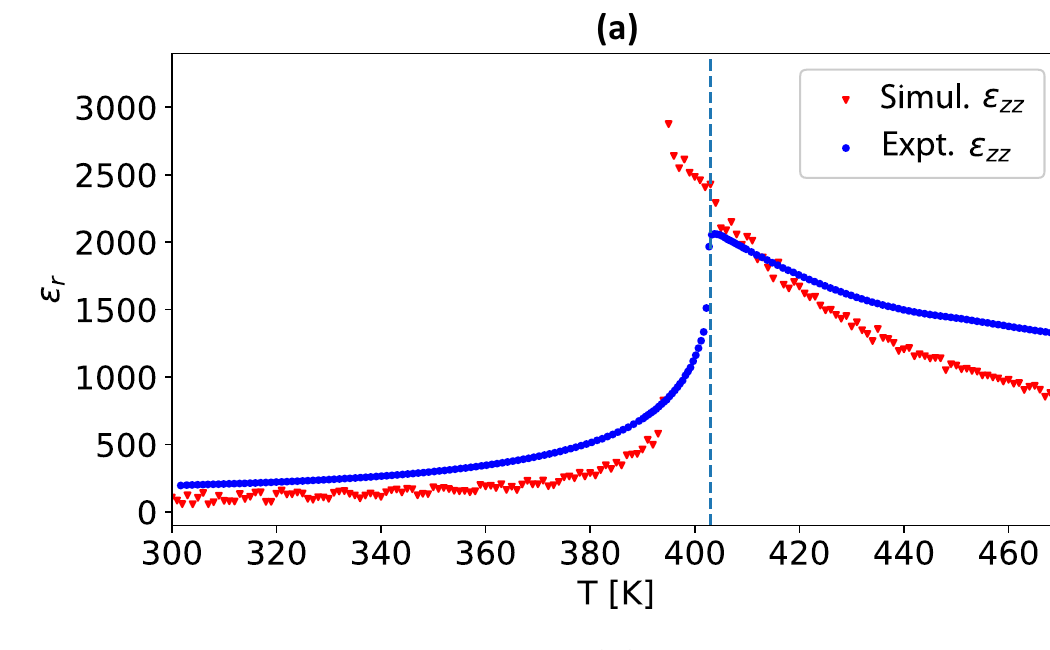
\includegraphics[height=2.85cm]{mayer2022_fig3a_permittivity.png}
      \vspace{0.04cm}

      {\fontsize{8.2}{9.7}\selectfont
      La dynamique moléculaire reproduit la tendance expérimentale autour de
      $T_C\simeq403\,$K.}

    \column{0.59\textwidth}
      \centering
      \tagline{Teal}{Ce stage : fermeture SCHA}\par
      \vspace{0.05cm}
      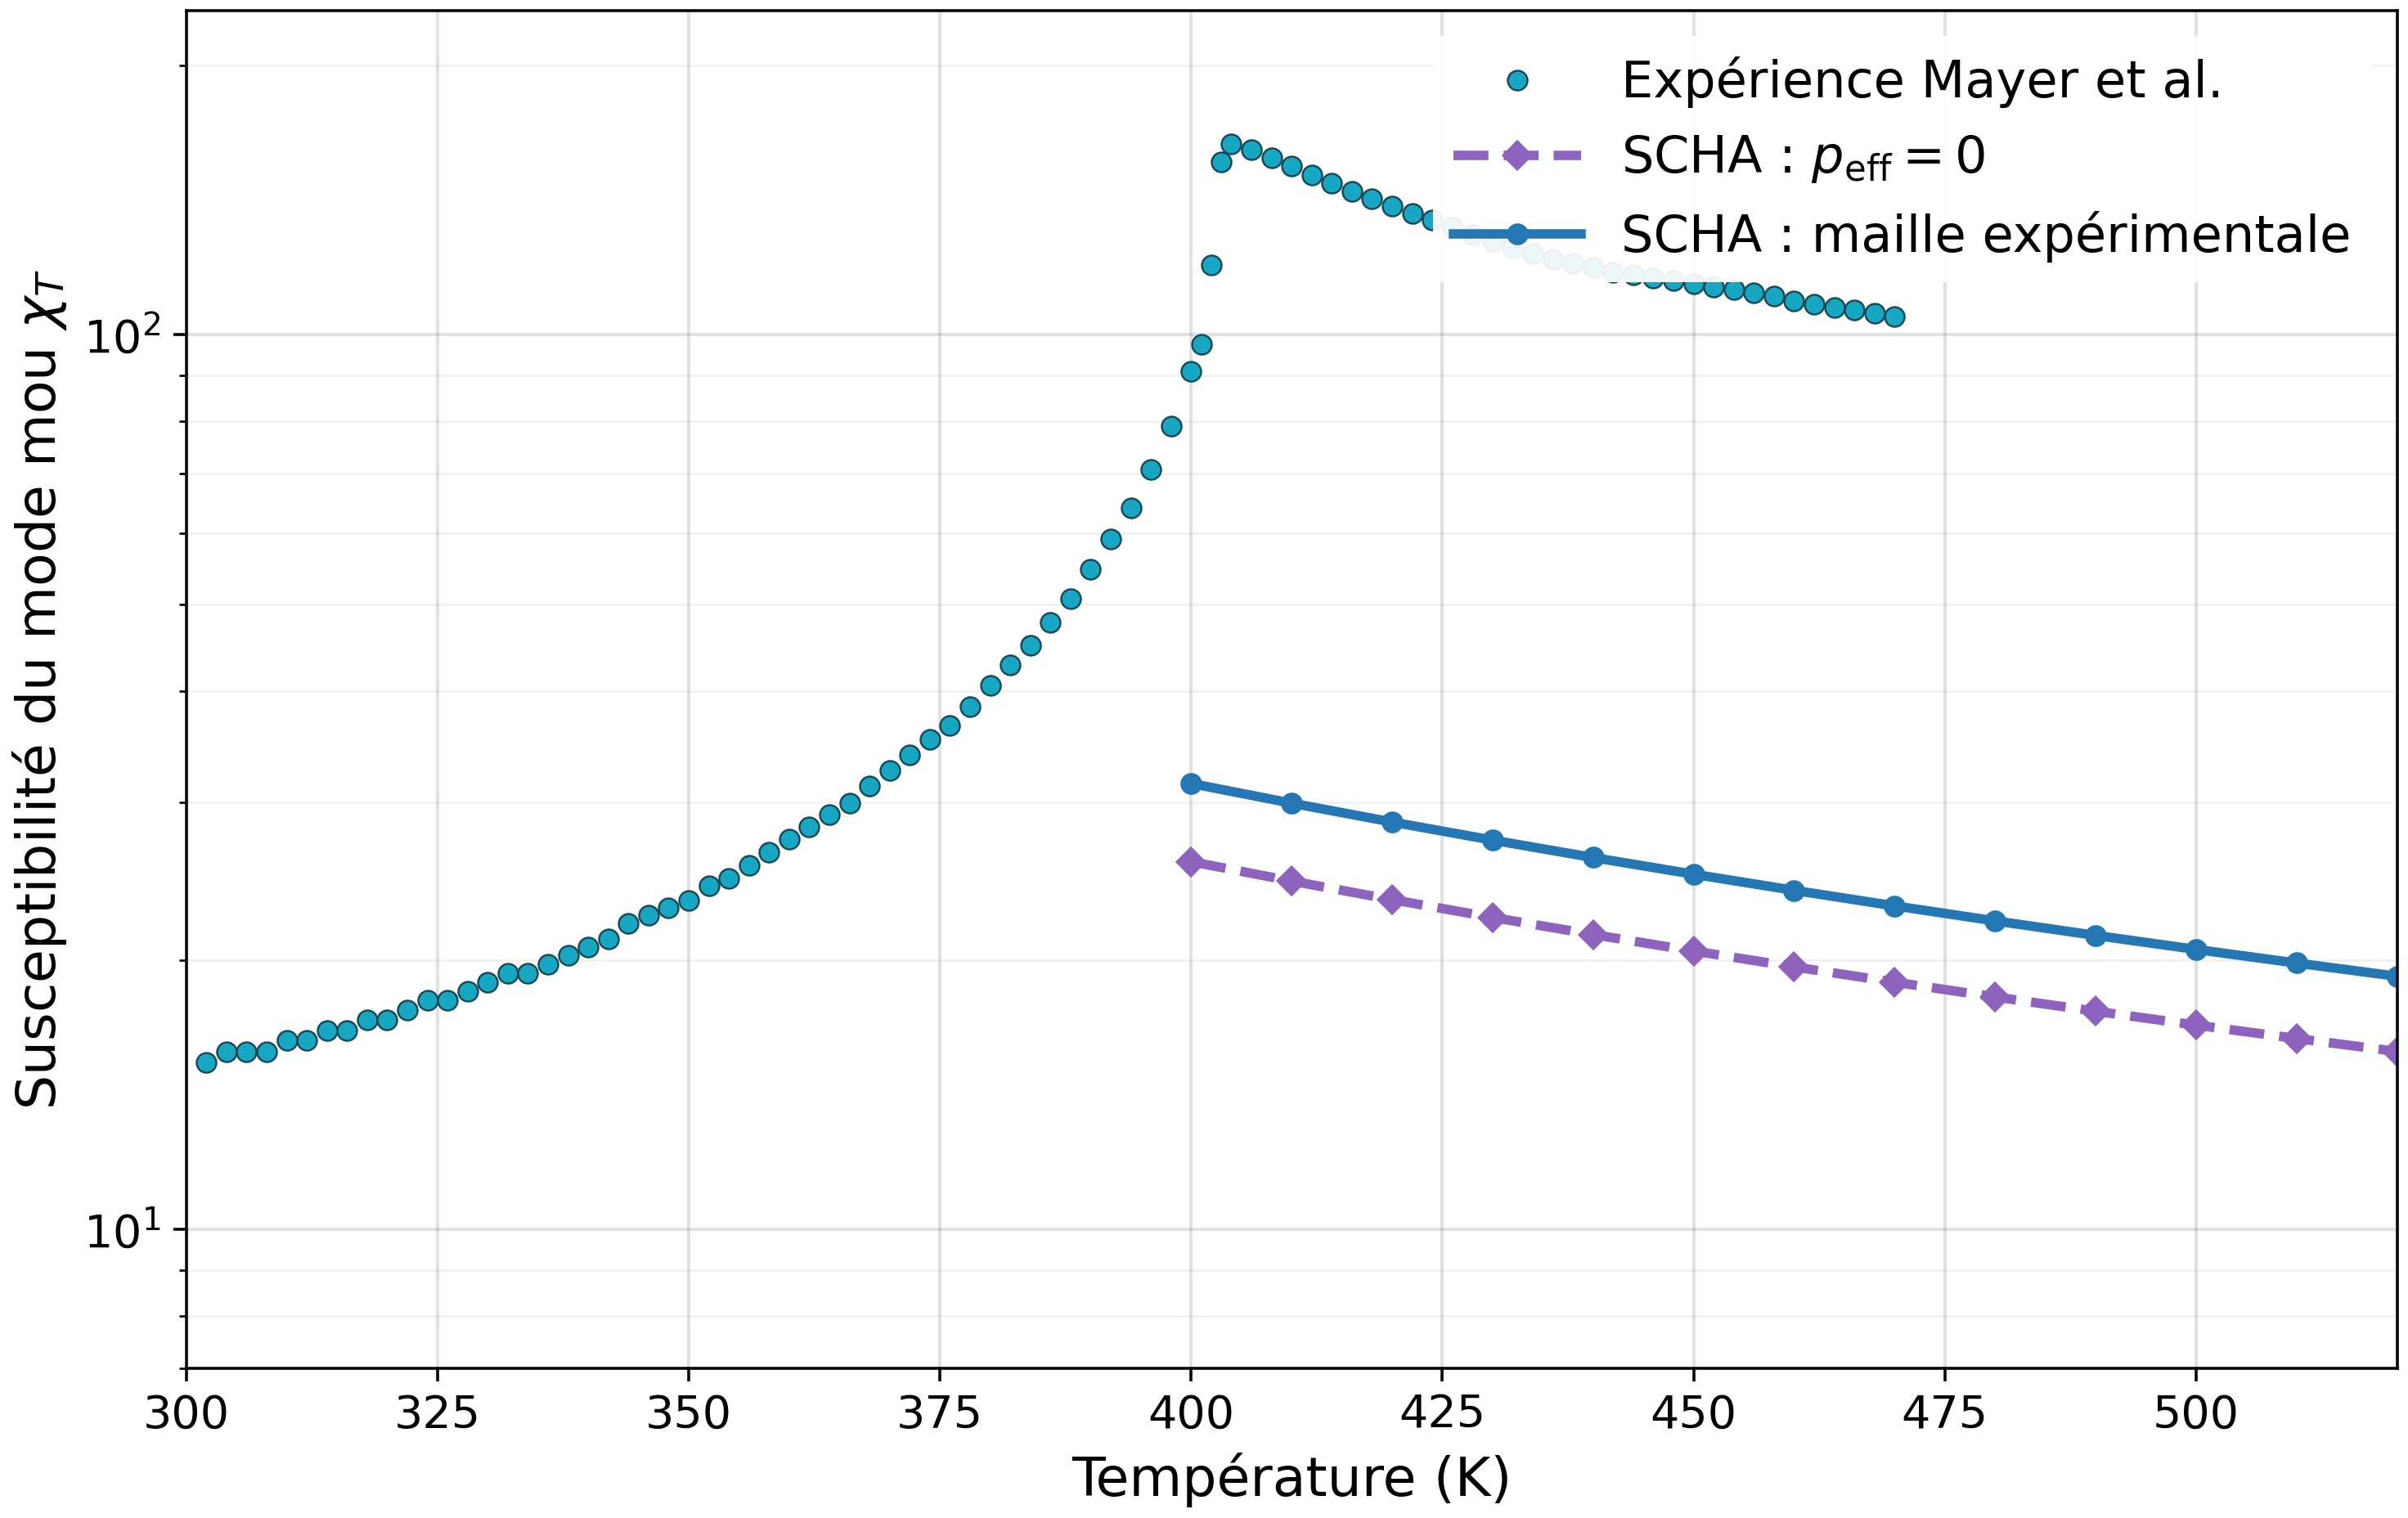
\includegraphics[height=3.70cm]{mayer_scha_slide_simplified.png}
      \vspace{0.04cm}

      {\fontsize{8.2}{9.7}\selectfont
      Avec le potentiel anharmonique de Mayer, la réponse SCHA reste sous
      les points de Mayer.}
  \end{columns}

  \vspace{-0.02cm}
  \begin{beamercolorbox}[wd=\linewidth,rounded=true,sep=0.22em]{block body}
    \centering\color{DeepNavy}\bfseries\fontsize{9.5}{11.2}\selectfont
    Potentiel anharmonique commun ; ancrage harmonique et fermeture explicités dans le rapport.
  \end{beamercolorbox}
  \vspace{-0.15cm}
  \source{calcul du stage, tables de la pipeline ; Mayer et al., \textit{Phys. Rev. B} 106, 064108 (2022), Fig.~3(a), CC BY 4.0.}
\end{frame}

\begin{frame}{Post-SCHA : isoler la première correction}
  \begin{columns}[c,onlytextwidth]
    \column{0.53\textwidth}
      \tagline{CSOrange}{Réorganisation autour de la SCHA}\par
      \vspace{0.08cm}
      \begin{beamercolorbox}[rounded=true,sep=0.40em]{block body}
        \centering
        {\fontsize{10.6}{12.8}\selectfont
          \(\displaystyle\begin{aligned}
            H={}&H_{\mathrm{SCHA}}+\epsilon\,\Delta V_{\mathrm{SCHA}},\\[-0.08cm]
            \Delta V_{\mathrm{SCHA}}={}&V(\mathbf P)
            +\frac12\mathbf P\!\cdot\!(A_0-A_{\mathrm{SCHA}})\!\cdot\!\mathbf P
          \end{aligned}\)}
        \par\vspace{0.08cm}
        {\color{Slate}\fontsize{8.2}{9.8}\selectfont
          \(A_0\) : noyau nu ; \(\epsilon=1\) restitue le Hamiltonien exact.}
      \end{beamercolorbox}
      \vspace{0.10cm}
      \begin{itemize}\setlength\itemsep{0.11cm}
        \item La partie non perturbée définit la référence gaussienne
              $H_{\mathrm{SCHA}}$.
        \item $\Delta V_{\mathrm{SCHA}}$ contient le contre-terme
              quadratique et l'anharmonicité.
        \item Hartree est déjà resommé dans $A_{\mathrm{SCHA}}$ :
              seules les corrections nouvelles sont ajoutées.
      \end{itemize}
    \column{0.42\textwidth}
      \centering
      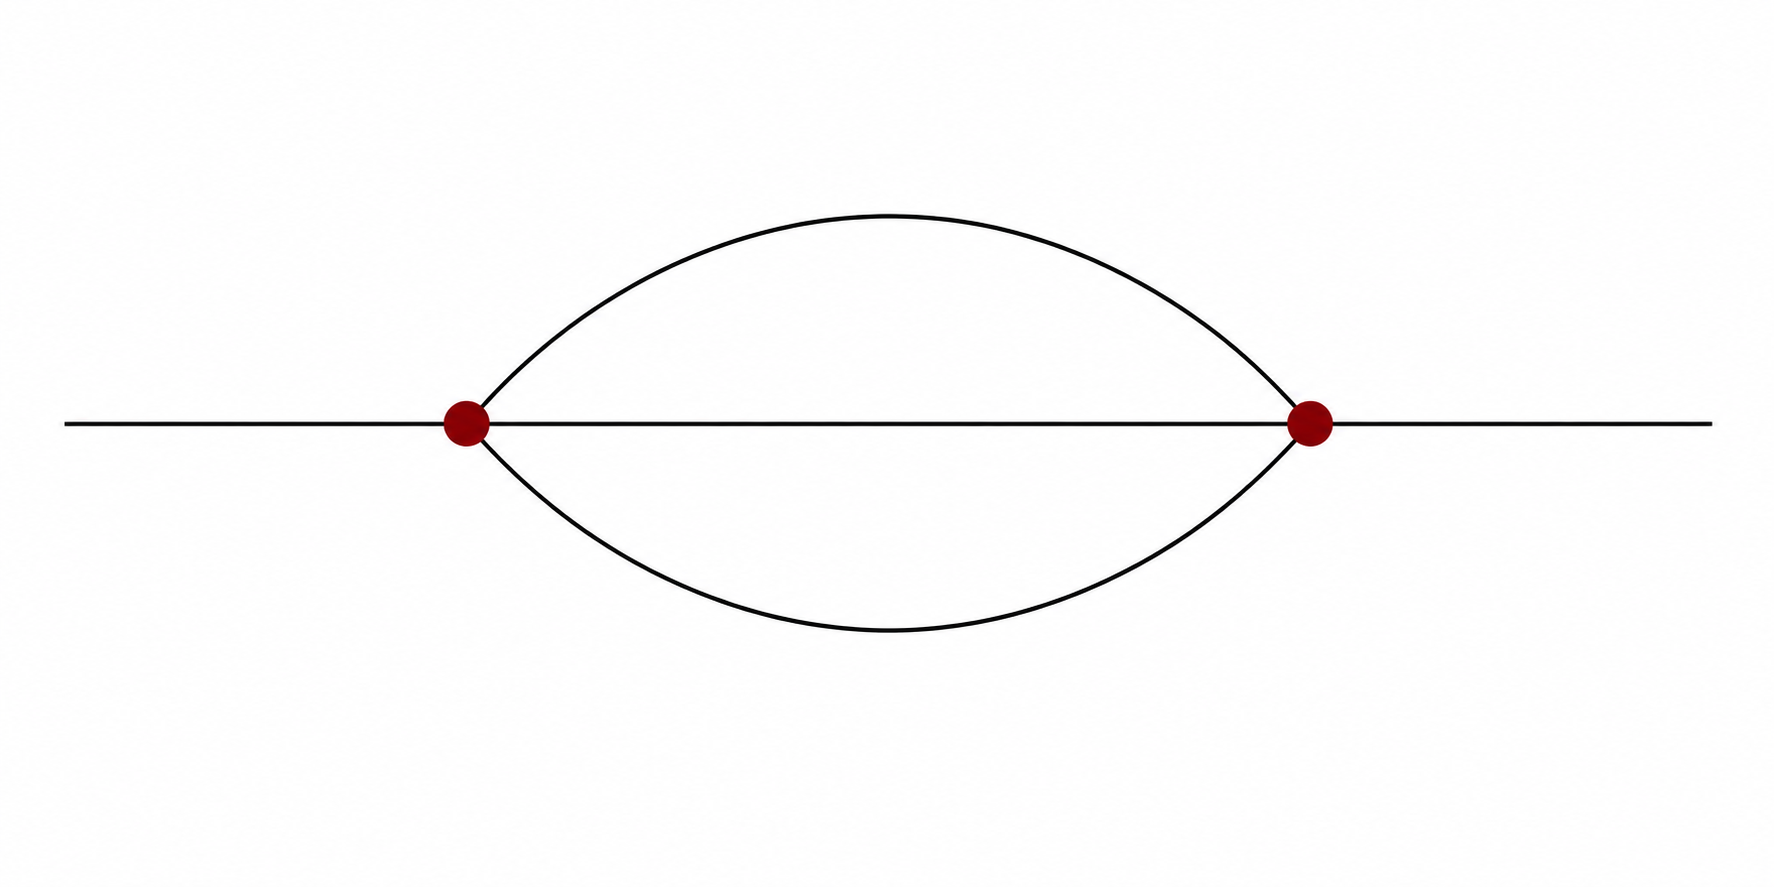
\includegraphics[width=0.96\linewidth]{sunset_post_scha.png}
      \vspace{-0.08cm}

      {\color{Teal}\bfseries Premier diagramme 1PI nouveau : le \emph{sunset} quartique.\par}
      \vspace{0.04cm}
      {\fontsize{8.4}{10.0}\selectfont
        deux vertices \(\overline\Gamma_4\), trois propagateurs
        \(G_{\mathrm{SCHA}}\).}
  \end{columns}
  \source{développement post-SCHA du stage ; diagramme \emph{sunset} généré pour la soutenance.}
\end{frame}

\begin{frame}[label=qa-post-scha-one-shot]{Post-SCHA : limites du diagnostic}
  \begin{columns}[c,onlytextwidth]
    \column{0.58\textwidth}
      \centering
      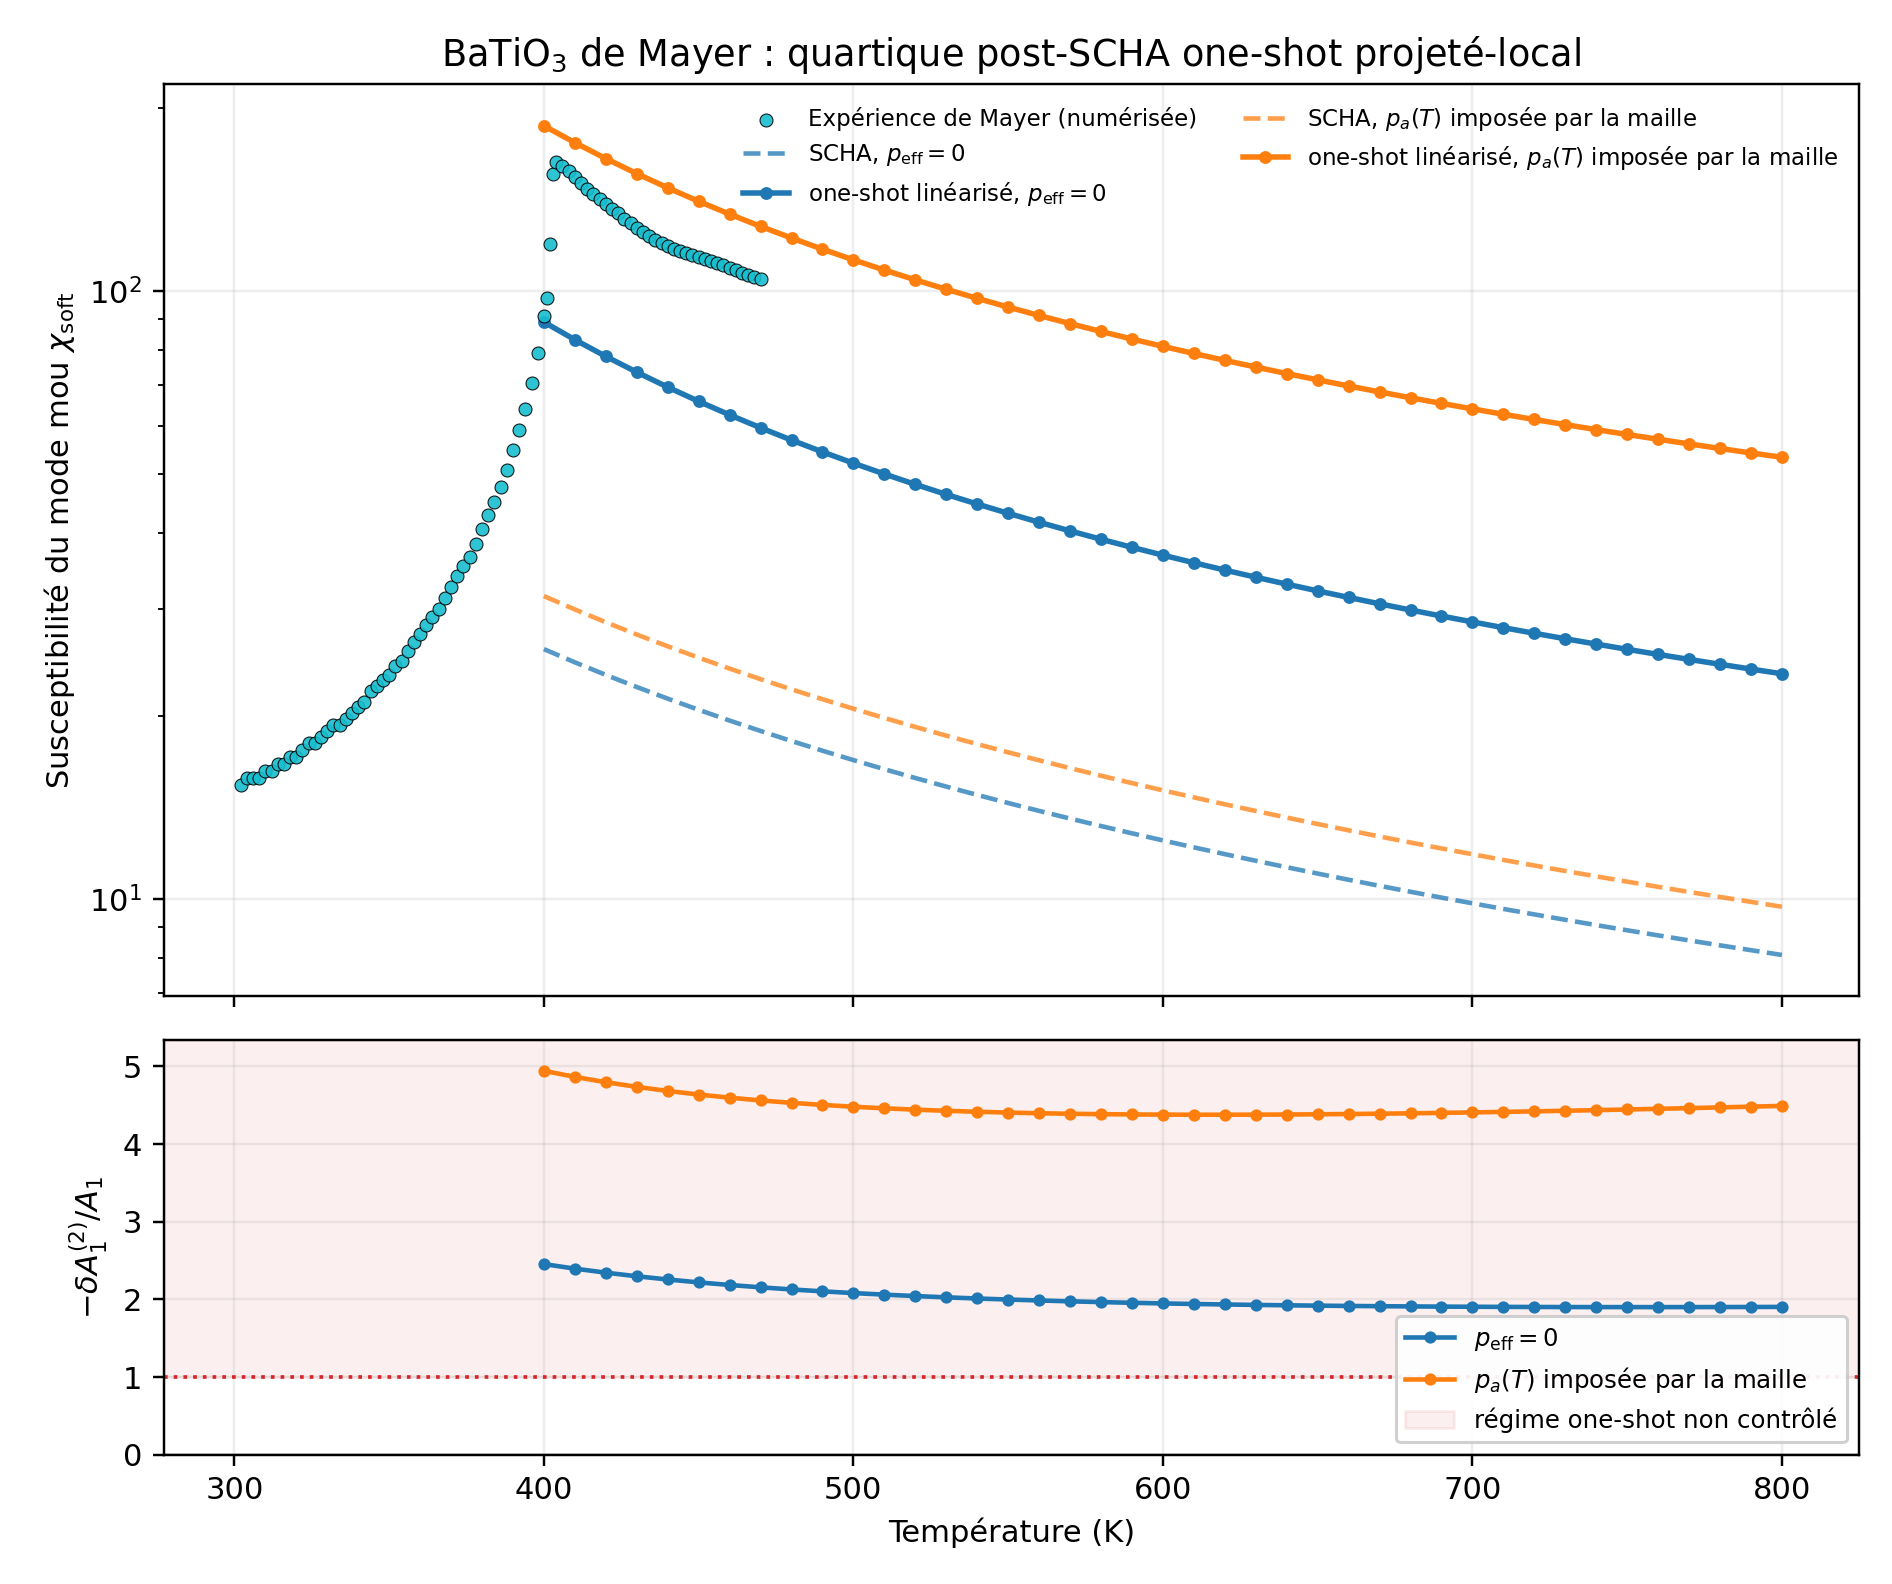
\includegraphics[height=4.15cm]{mayer_post_scha_quartic_one_shot_400_800K_n40.png}
    \column{0.38\textwidth}
      \tagline{CSOrange}{Deux indices convergents}\par
      \vspace{0.08cm}
      {\fontsize{8.7}{10.4}\selectfont
      \textbf{Mayer :} les modes optiques éliminés renormalisent le mode mou.\par
      \vspace{0.08cm}
      \textbf{Perturbation :} le \emph{sunset} quartique déplace la réponse vers les données de Mayer.}
      \vspace{0.08cm}

      \begin{beamercolorbox}[rounded=true,sep=0.30em]{block body}
        \centering
        {\color{CSOrange}\bfseries Réserve indispensable}\par
        \vspace{0.02cm}
        \(\displaystyle
          -\frac{\delta A_1^{(2)}}{A_1}>1
        \)
        \par\vspace{0.02cm}
        {\fontsize{8.2}{9.8}\selectfont
          sur tout l'intervalle : le développement \emph{one-shot} n'est pas contrôlé.}
      \end{beamercolorbox}
      \vspace{0.05cm}

      {\color{Teal}\fontsize{8.5}{10.1}\selectfont\bfseries
      Réexaminer la fermeture SCHA centrée et sa réponse.}
  \end{columns}
  \vspace{-0.10cm}
  \source{calcul du stage ; diagnostic quartique projeté-local \emph{one-shot}, paramètres de Mayer et al. (2022).}
\end{frame}

\begin{frame}{VCA--SCHA : cristaux virtuels}
  \begin{columns}[T,onlytextwidth]
    \column{0.47\textwidth}
      \tagline{CSOrange}{1. Interpoler les entrées microscopiques}\par
      \vspace{0.06cm}
      \begin{beamercolorbox}[rounded=true,sep=0.34em]{block body}
        \centering
        \[
          \lambda_{\rm VCA}(x)
          =x\lambda_{\rm BTO}+(1-x)\lambda_{\rm STO}
        \]
      \end{beamercolorbox}
      \vspace{0.12cm}
      {\small Paramètres indépendants : potentiel local, interactions à courte
      portée, élasticité et couplages mode--déformation.}

    \column{0.49\textwidth}
      \tagline{Teal}{2. Reconstruire les quantités dépendantes}\par
      \vspace{0.06cm}
      \begin{beamercolorbox}[rounded=true,sep=0.28em]{block body}
        \centering
        {\fontsize{8.4}{10.0}\selectfont
        $\Omega_0(x)=a_0(x)^3$,
        \qquad
        $D(x)\propto\dfrac{Z^*(x)^2}
        {\varepsilon_\infty(x)\Omega_0(x)}$\par
        \vspace{0.10cm}
        $\displaystyle
        A_{0,\rm VCA}(\bm q;x)
        =xA_{0,\rm BTO}^{\rm nd}(\bm q)
        +(1-x)A_{0,\rm STO}^{\rm nd}(\bm q)
        +D_{\rm VCA}(\bm q;x)$.}
      \end{beamercolorbox}
  \end{columns}

  \vspace{0.15cm}
  \begin{columns}[c,onlytextwidth]
    \column{0.56\textwidth}
      \tagline{WarmGold}{Ce que cette étape démontre}\par
      \vspace{0.04cm}
      La VCA conserve la translation :
      $A(\bm k,\bm k';x)=\delta_{\bm k\bm k'}A(\bm k;x)$.
      Chaque $\bm k$ reste donc une matrice $3\times3$ dans le solveur existant :
      la chaîne de calcul s'applique aux cristaux virtuels.
    \column{0.40\textwidth}
      \begin{beamercolorbox}[rounded=true,sep=0.40em]{block body}
        \centering\bfseries
        Illustration de méthode : le modèle reste non prédictif pour
        BaTiO$_3$, donc aussi pour le BST à ce stade.
      \end{beamercolorbox}
  \end{columns}
  \vspace{-0.03cm}
  \source{développement du stage ; section « Virtual crystal approximation » de \textit{Maxime notes}.}
\end{frame}

\begin{frame}[label=qa-bst]{BST : illustration}
  \centering
  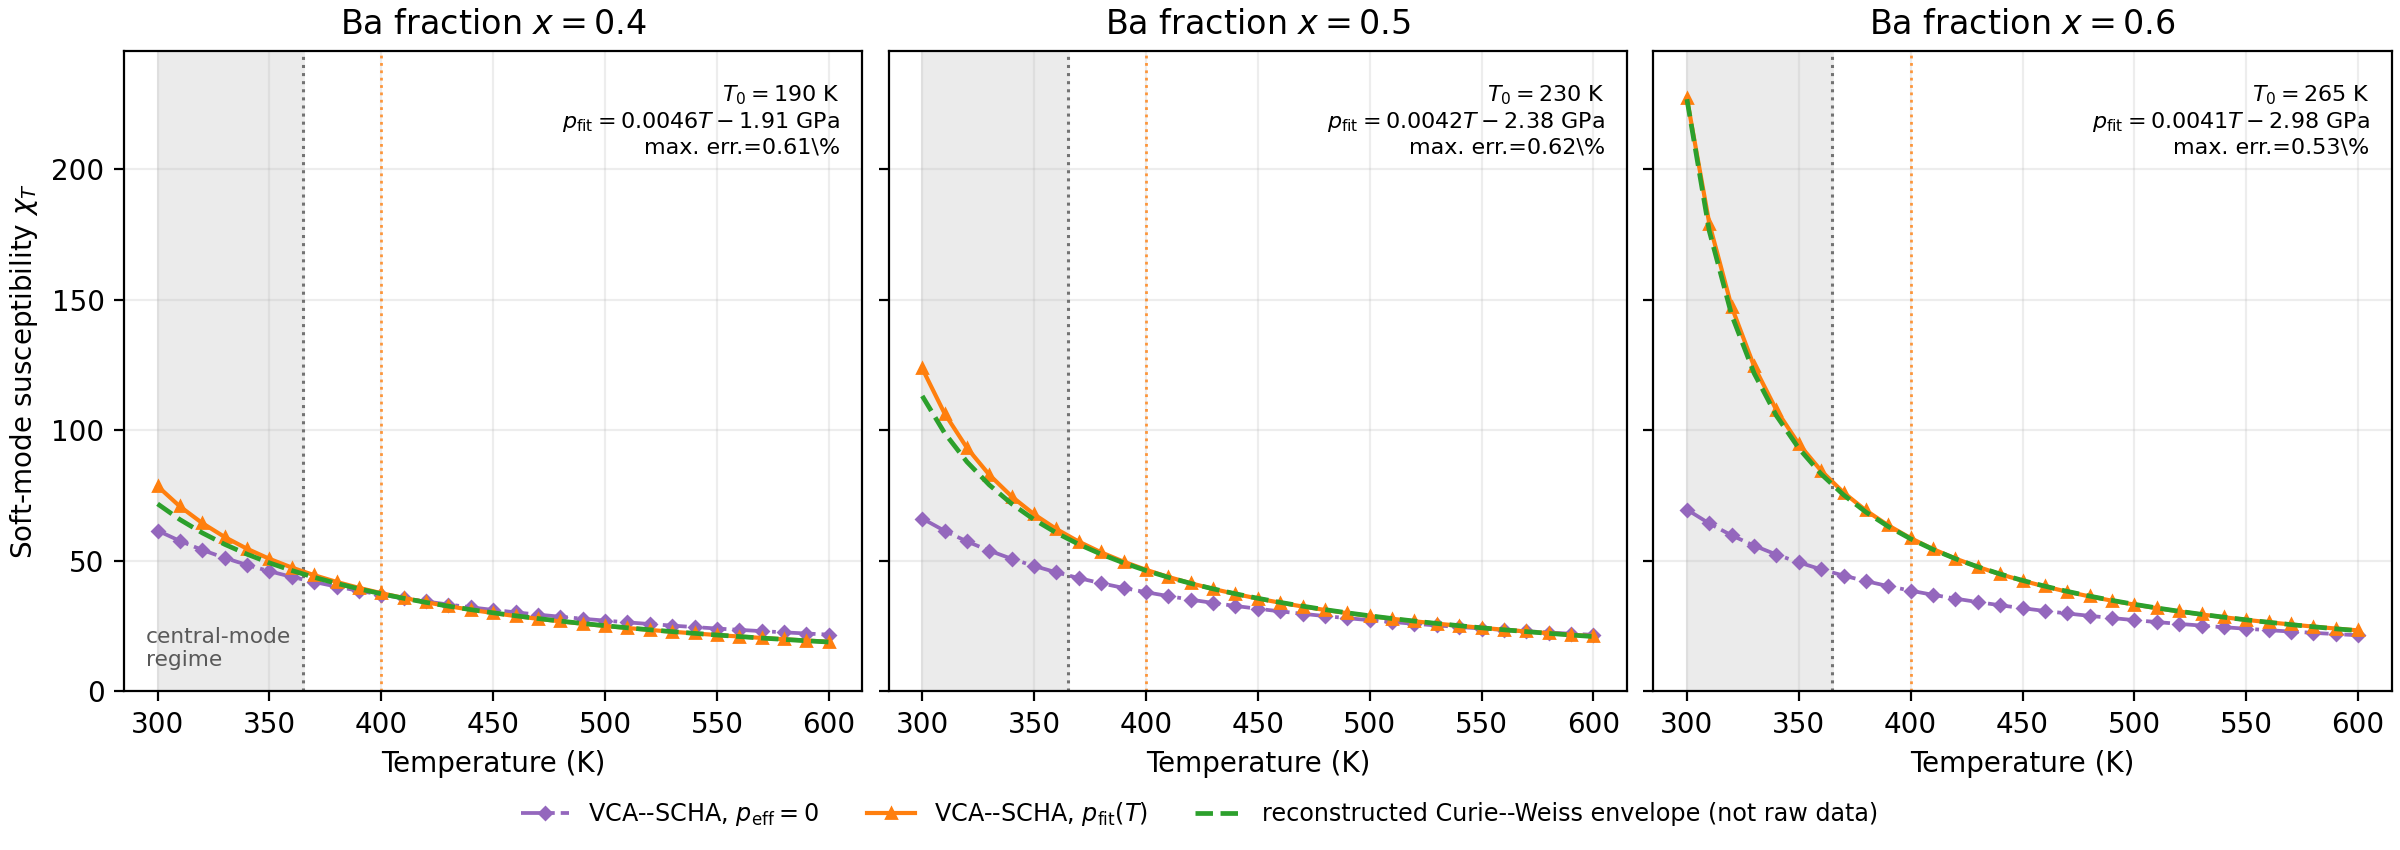
\includegraphics[width=0.84\linewidth]{chi_temperature_bst_vca_x040_060_300_600K_n40.png}
  \vspace{-0.08cm}

  \begin{columns}[T,onlytextwidth]
    \column{0.49\textwidth}
      {\fontsize{7.8}{9.1}\selectfont
      \tagline{CSOrange}{Objet de la figure :}
      VCA--SCHA pour plusieurs compositions $x$. La cible verte est reconstruite
      par $\varepsilon_r^{\rm ref}=C/(T-T_0)$ : aucun point brut n'est affiché.}
    \column{0.47\textwidth}
      {\fontsize{7.8}{9.1}\selectfont
      \tagline{Teal}{Statut des courbes :}
      violet $=$ VCA--SCHA ; orange $=$ calibration inverse sur la cible.
      La non-prédictivité pour BaTiO$_3$ interdit d'interpréter ce tracé
      comme une prédiction du BST.}
  \end{columns}
  \vspace{-0.10cm}
  \source{calcul du stage ; référence verte reconstruite d'après Weerasinghe et al. (2013), sans points bruts.}
\end{frame}

% =============================================================================
% BILAN DE STAGE ET PRISE DE RECUL
% =============================================================================

\section{Bilan et suite}

% Slide 24 mise en réserve temporairement.
\iffalse
\begin{frame}{Le stage a produit des livrables réutilisables}
  \begin{columns}[T,onlytextwidth]
    \column{0.48\textwidth}
      \begin{block}{Socle scientifique}
        \begin{itemize}\setlength\itemsep{0.14cm}
          \item notes LaTeX structurées : réseau $\to$ continu $\to$ SCHA $\to$ réponse ;
          \item normalisations, tenseurs et élimination des déformations explicités ;
          \item extensions paraélectrique, ferroélectrique et piézoélectrique.
        \end{itemize}
      \end{block}
    \column{0.48\textwidth}
      \begin{block}{Socle numérique}
        \begin{itemize}\setlength\itemsep{0.14cm}
          \item solveurs Python paraélectrique et ferroélectrique ;
          \item noyaux périodiques, sommes de Matsubara et contrôles de stabilité ;
          \item sorties CSV/JSON et figures reproductibles.
        \end{itemize}
      \end{block}
  \end{columns}
  \vspace{0cm}
  \begin{columns}[T,onlytextwidth]
    \column{0.31\textwidth}\metric[CSOrange]{4\,300+}{lignes de notes de calcul consolidées}
    \column{0.31\textwidth}\metric[Teal]{2 phases}{paraelectrique et ferroélectrique}
    \column{0.31\textwidth}\metric[WarmGold]{3 matériaux}{BaTiO$_3$, SrTiO$_3$, base pour BST}
  \end{columns}
\end{frame}
\fi

% Slide 25 fusionnée avec la conclusion et mise en réserve temporairement.
\iffalse
\begin{frame}{La suite se priorise par gain scientifique et effort}
  \begin{tikzpicture}[
      stage/.style={rounded corners=2pt,minimum height=1.20cm,text width=3.65cm,align=left,inner sep=0.30cm},
      arr/.style={-{Latex[length=2.5mm]},very thick,Slate}
    ]
    \node[stage,fill=PaleOrange,text=DeepNavy] (s1) at (0,0) {\textbf{1. Fiabiliser}\newline Comparer les énergies libres des branches et automatiser les tests de convergence.};
    \node[stage,fill=PaleTeal,text=DeepNavy] (s2) at (4.55,0) {\textbf{2. Enrichir}\newline Ajouter les modes optiques manquants et la rotation d'oxygène de SrTiO$_3$.};
    \node[stage,fill=PaleGold,text=DeepNavy] (s3) at (9.10,0) {\textbf{3. Exploiter}\newline Valider sur davantage de mesures puis interpoler la composition Ba/Sr.};
    \draw[arr] (s1) -- (s2);
    \draw[arr] (s2) -- (s3);
  \end{tikzpicture}
  \vspace{0.62cm}
  \begin{columns}[T,onlytextwidth]
    \column{0.48\textwidth}
      \begin{block}{Valeur pour le SPMS}
        Disposer d'un intermédiaire analytique entre calculs DFT, simulations lourdes et mesures.
      \end{block}
    \column{0.48\textwidth}
      \begin{block}{Décision avant extension BST}
        Vérifier que le modèle enrichi reproduit simultanément volume, $T_C$ et $\chi(T)$ sans paramètre non physique.
      \end{block}
  \end{columns}
\end{frame}
\fi

% Slide 26 mise en réserve temporairement.
\iffalse
\begin{frame}{Compétences acquises et prise de recul professionnelle}
  \begin{columns}[T,onlytextwidth]
    \column{0.48\textwidth}
      \begin{block}{Compétences démontrées}
        \begin{itemize}\setlength\itemsep{0.15cm}
          \item reformuler un problème ouvert en chaîne de calcul ;
          \item articuler physique, mathématiques et implémentation ;
          \item construire des contrôles plutôt que valider « à l'œil » ;
          \item expliquer une limite technique sans masquer l'incertitude.
        \end{itemize}
      \end{block}
    \column{0.48\textwidth}
      \begin{block}{Éthique et développement durable}
        \begin{itemize}\setlength\itemsep{0.15cm}
          \item calibration et ajustement diagnostique clairement séparés ;
          \item données, sources et hypothèses traçables ;
          \item calcul déterministe ciblé, sans échantillonnage stochastique massif ;
          \item coût en $n^3$ de la grille suivi : la sobriété reste un compromis, pas un slogan.
        \end{itemize}
      \end{block}
  \end{columns}
  \vspace{0.12cm}
  {\color{DeepNavy}\bfseries Compétence centrale : rendre une modélisation complexe auditable par quelqu'un d'autre.}
\end{frame}
\fi

{
\setbeamerfont{frametitle}{series=\bfseries,size=\fontsize{16.5}{19}}
\begin{frame}{Conclusion : améliorer la méthode avant l'extension}
  \centering
  \vspace{-0.04cm}
  \begin{tikzpicture}[x=1cm,y=1cm,
      stop/.style={rounded corners=3pt,minimum width=3.34cm,minimum height=1.02cm,
        align=center,inner sep=0.16cm,font=\fontsize{8.4}{9.8}\selectfont,
        text=DeepNavy,draw=white,line width=0.8pt},
      num/.style={circle,minimum size=0.48cm,inner sep=0pt,font=\bfseries\scriptsize,
        text=white,draw=white,line width=0.7pt},
      future/.style={rounded corners=4pt,minimum width=8.25cm,minimum height=0.94cm,
        align=center,inner sep=0.15cm,fill=bordeauCS,text=white,
        font=\fontsize{8.6}{10.0}\selectfont\bfseries}
    ]
    % Le ruban est tracé avant les étapes : il forme un unique chemin en S.
    \draw[Slate!32,line width=8.2pt,rounded corners=16pt]
      (1.55,4.05) -- (10.55,4.05)
      to[out=0,in=0] (10.55,2.28) -- (1.55,2.28)
      to[out=180,in=180] (1.55,0.64) -- (3.48,0.64);
    \draw[-{Latex[length=3.0mm,width=2.4mm]},white,line width=2.1pt,
      rounded corners=16pt]
      (1.55,4.05) -- (10.55,4.05)
      to[out=0,in=0] (10.55,2.28) -- (1.55,2.28)
      to[out=180,in=180] (1.55,0.64) -- (3.48,0.64);

    \node[stop,fill=PaleOrange] (s1) at (1.70,4.05)
      {Paramètres \textit{ab initio}\\$\Downarrow$ Hamiltonien effectif};
    \node[stop,fill=Mist] (s2) at (6.05,4.05)
      {Réseau $\longrightarrow$ champ continu\\$\bm P(\bm r,\tau)$};
    \node[stop,fill=PaleTeal] (s3) at (10.40,4.05)
      {Thermique + quantique\\$\Downarrow$ SCHA $\Downarrow\ \chi(T)$};

    \node[stop,fill=PaleGold] (s4) at (10.40,2.28)
      {Déformations acoustiques\\effet mesurable};
    \node[stop,fill=Mist] (s5) at (6.05,2.28)
      {BaTiO$_3$ puis BST\\confrontation aux mesures};
    \node[stop,fill=PaleOrange] (s6) at (1.70,2.28)
      {Diagnostic\\la SCHA reste trop rigide};

    \foreach \n/\x/\y/\c in {
      1/0.30/4.55/CSOrange,2/4.65/4.55/Slate,3/9.00/4.55/Teal,
      4/11.80/2.78/WarmGold,5/7.45/2.78/Slate,6/3.10/2.78/CSOrange}{
      \node[num,fill=\c] at (\x,\y) {\n};
    }

    \node[future] (next) at (7.55,0.64)
      {LA SUITE : contrôler la post-SCHA $\;\longrightarrow\;$ enrichir les modes
       $\;\longrightarrow\;$ valider un BST prédictif};
  \end{tikzpicture}

  \vspace{0.05cm}
  {\color{DeepNavy}\bfseries\fontsize{9.5}{11.2}\selectfont
    Le passage à l'étape suivante exige de reproduire ensemble
    le volume, $T_C$ et $\chi(T)$ sans contre-terme non physique.\par}
\end{frame}
}

\discussionbuttonenabledfalse
\begin{frame}[label=questions-discussion]{Questions et discussion}
  \centering

  \fontsize{8.7}{10.2}\selectfont
  \begin{columns}[T,onlytextwidth]
    \column{0.31\textwidth}
      \begin{minipage}[t][2.50cm][t]{\linewidth}
        \centering
        \hyperlink{qa-app}{%
          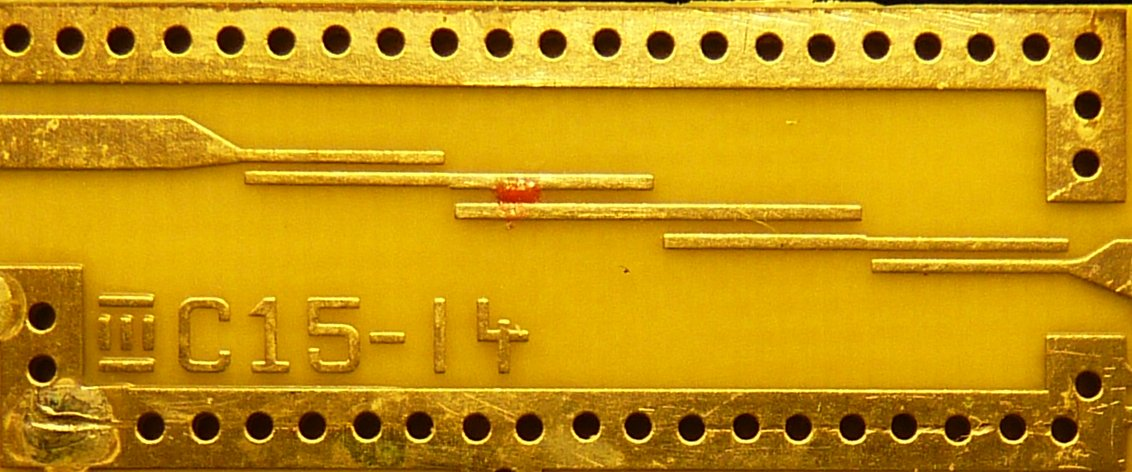
\includegraphics[width=\linewidth,height=1.46cm,keepaspectratio]
            {applications/microstrip_bandpass_filter.jpg}}
        \vspace{0.05cm}

        {\color{CSOrange}\bfseries Pourquoi choisir le BST ?\par}
        \vfill
        \hyperlink{qa-app}{\beamergotobutton{Revoir la slide 3}}
      \end{minipage}

    \column{0.31\textwidth}
      \begin{minipage}[t][2.50cm][t]{\linewidth}
        \centering
        \hyperlink{qa-quantum}{%
          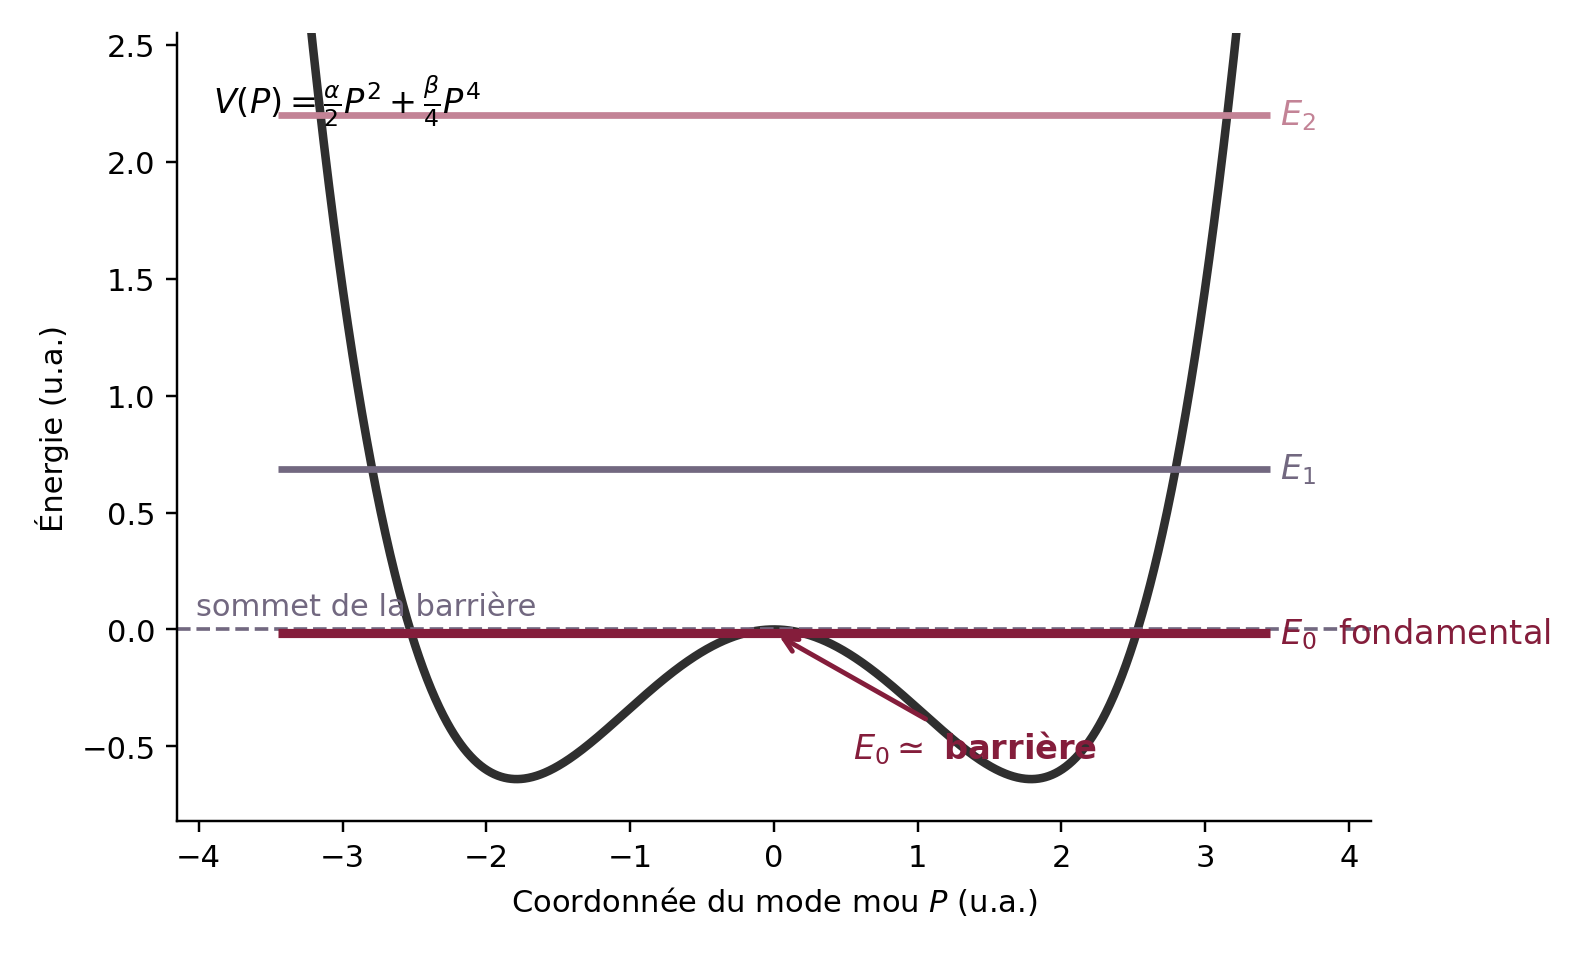
\includegraphics[width=\linewidth,height=1.46cm,keepaspectratio]
            {double_puit_niveaux.png}}
        \vspace{0.05cm}

        {\color{Teal}\bfseries Pourquoi intégrer le quantique ?\par}
        \vfill
        \hyperlink{qa-quantum}{\beamergotobutton{Revoir la slide 8}}
      \end{minipage}

    \column{0.31\textwidth}
      \begin{minipage}[t][2.50cm][t]{\linewidth}
        \centering
        \hyperlink{qa-scha}{%
          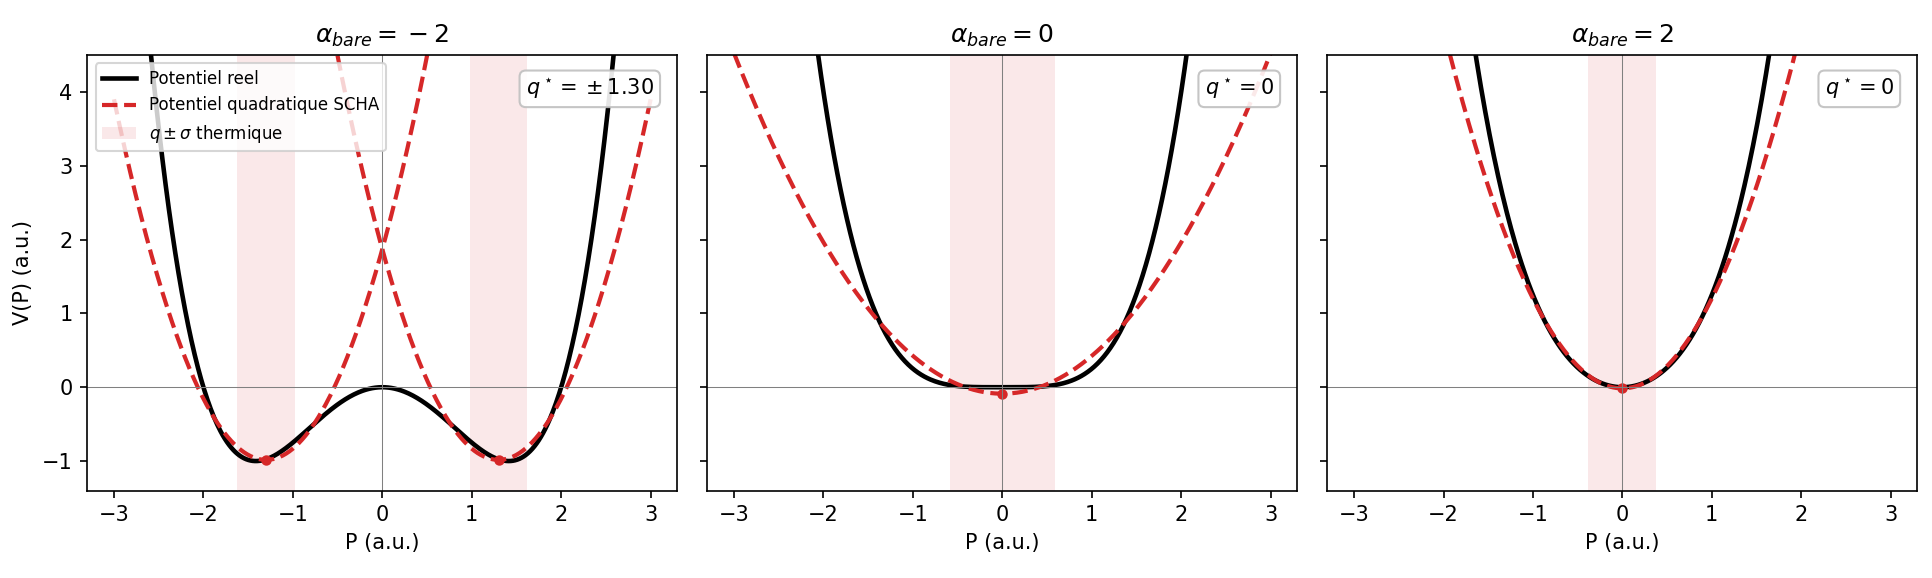
\includegraphics[width=\linewidth,height=1.46cm,keepaspectratio]
            {double_puit_scha.png}}
        \vspace{0.05cm}

        {\color{WarmGold}\bfseries Pourquoi la SCHA ?\par}
        \vfill
        \hyperlink{qa-scha}{\beamergotobutton{Revoir la slide 14}}
      \end{minipage}
  \end{columns}

  \vspace{0.18cm}

  \begin{columns}[T,onlytextwidth]
    \column{0.31\textwidth}
      \begin{minipage}[t][2.50cm][t]{\linewidth}
        \centering
        \hyperlink{qa-bto}{%
          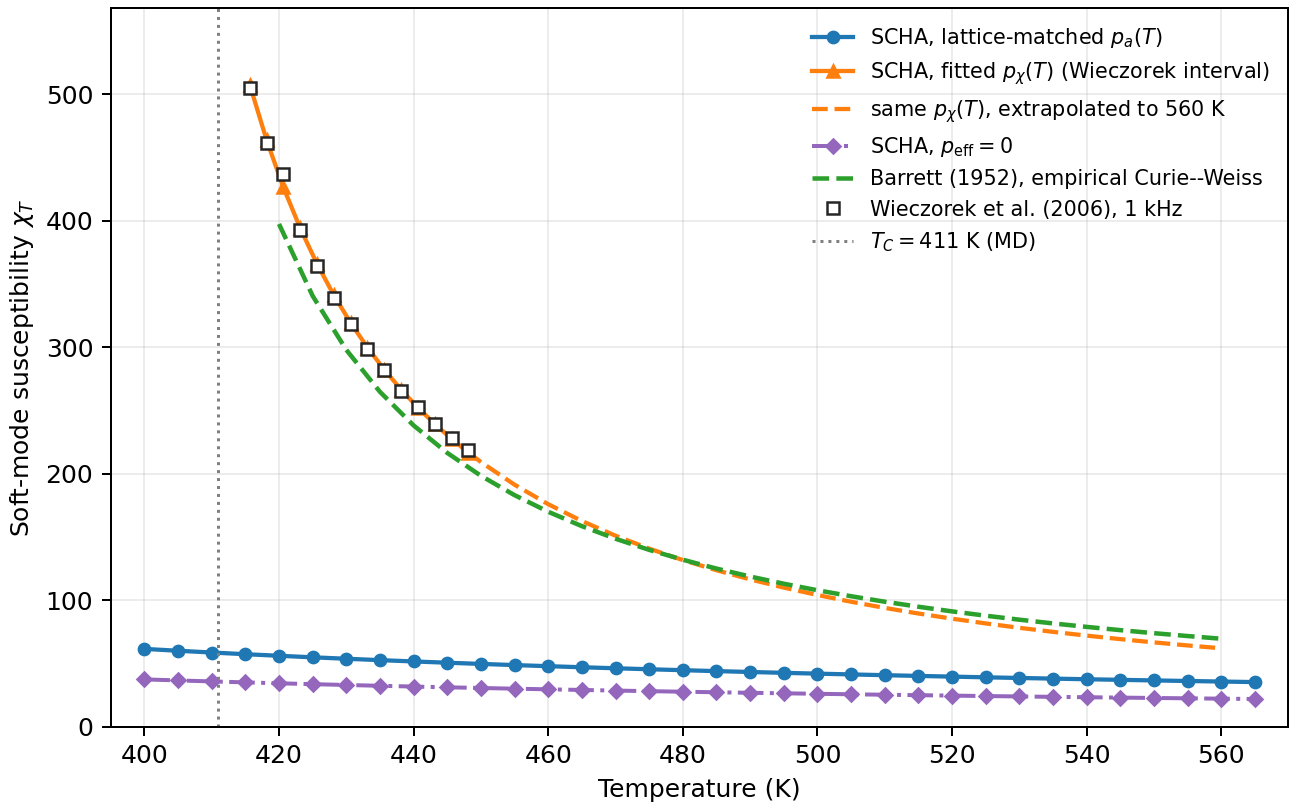
\includegraphics[width=\linewidth,height=1.46cm,keepaspectratio]
            {chi_temperature_400_565K_inhomogeneous_quartic.png}}
        \vspace{0.05cm}

        {\color{CSOrange}\bfseries Quel écart pour BaTiO$_3$ ?\par}
        \vfill
        \hyperlink{qa-bto}{\beamergotobutton{Revoir la slide 18}}
      \end{minipage}

    \column{0.31\textwidth}
      \begin{minipage}[t][2.50cm][t]{\linewidth}
        \centering
        \hyperlink{qa-missing}{%
          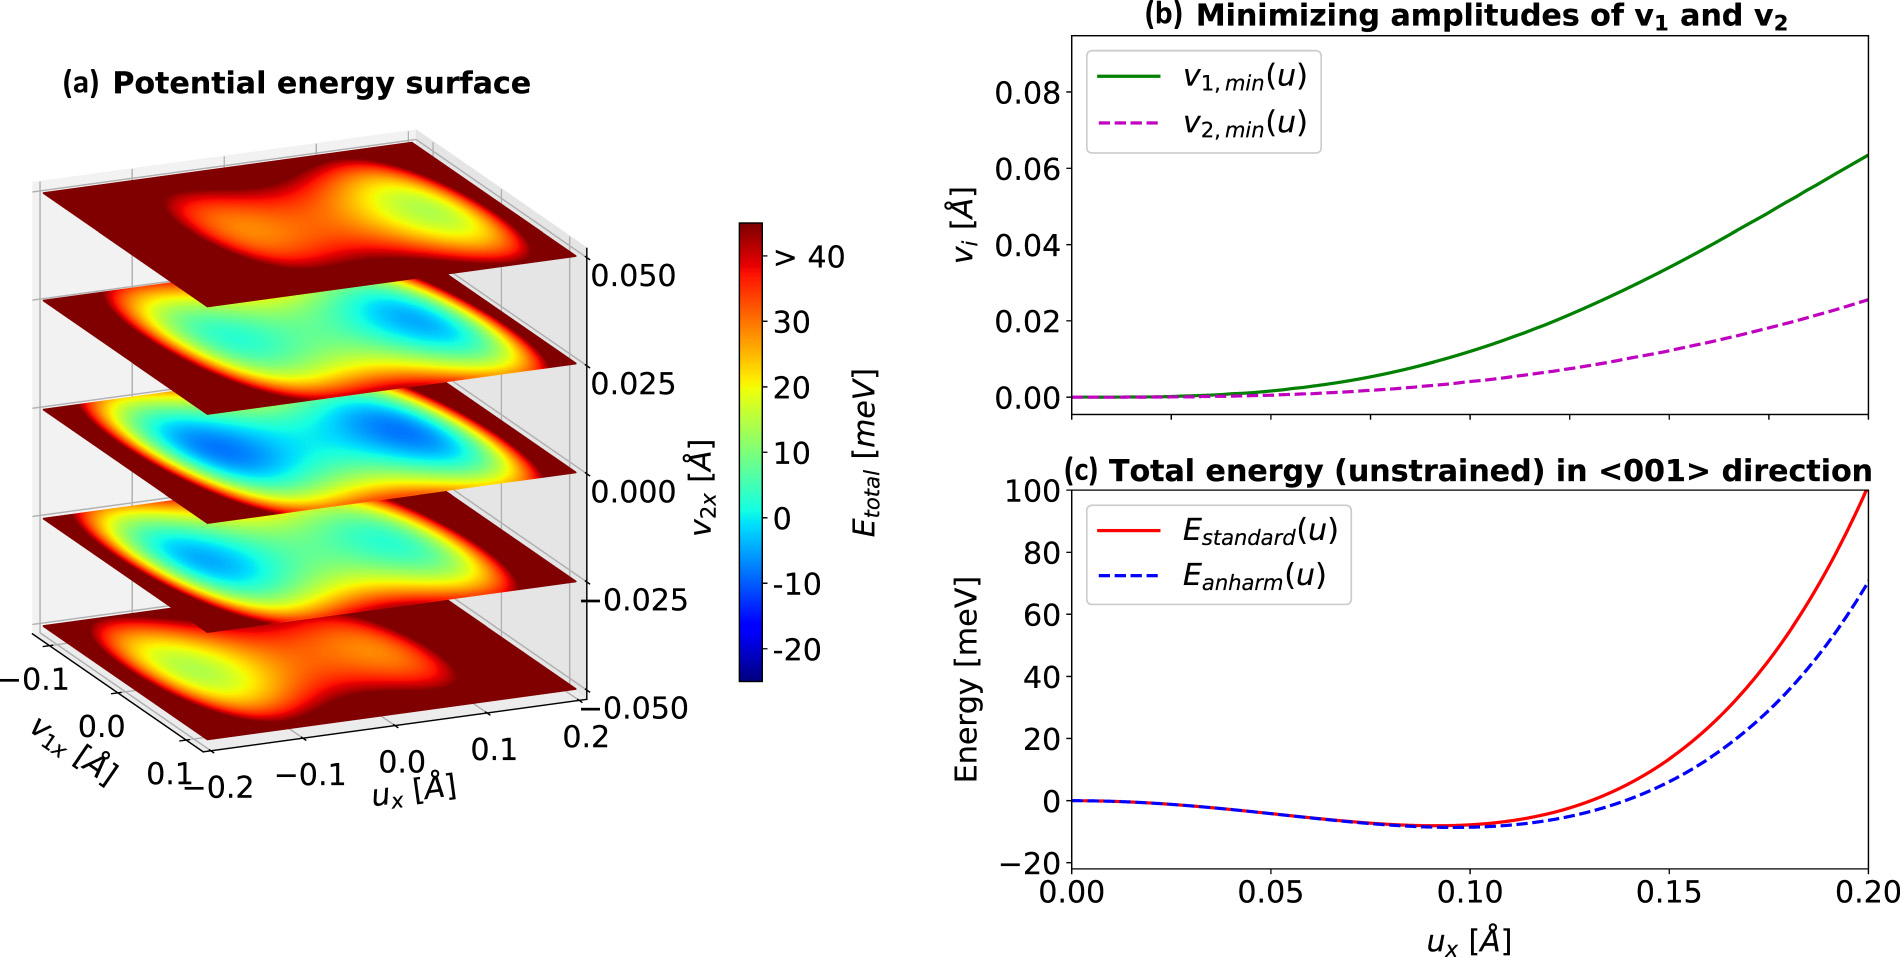
\includegraphics[width=\linewidth,height=1.46cm,keepaspectratio]
            {mayer2022_anharmonic_coupling_fig1.png}}
        \vspace{0.05cm}

        {\color{Teal}\bfseries Quels termes peuvent manquer ?\par}
        \vfill
        \hyperlink{qa-missing}{\beamergotobutton{Revoir la slide 20}}
      \end{minipage}

    \column{0.31\textwidth}
      \begin{minipage}[t][2.50cm][t]{\linewidth}
        \centering
        \hyperlink{qa-post-scha}{%
          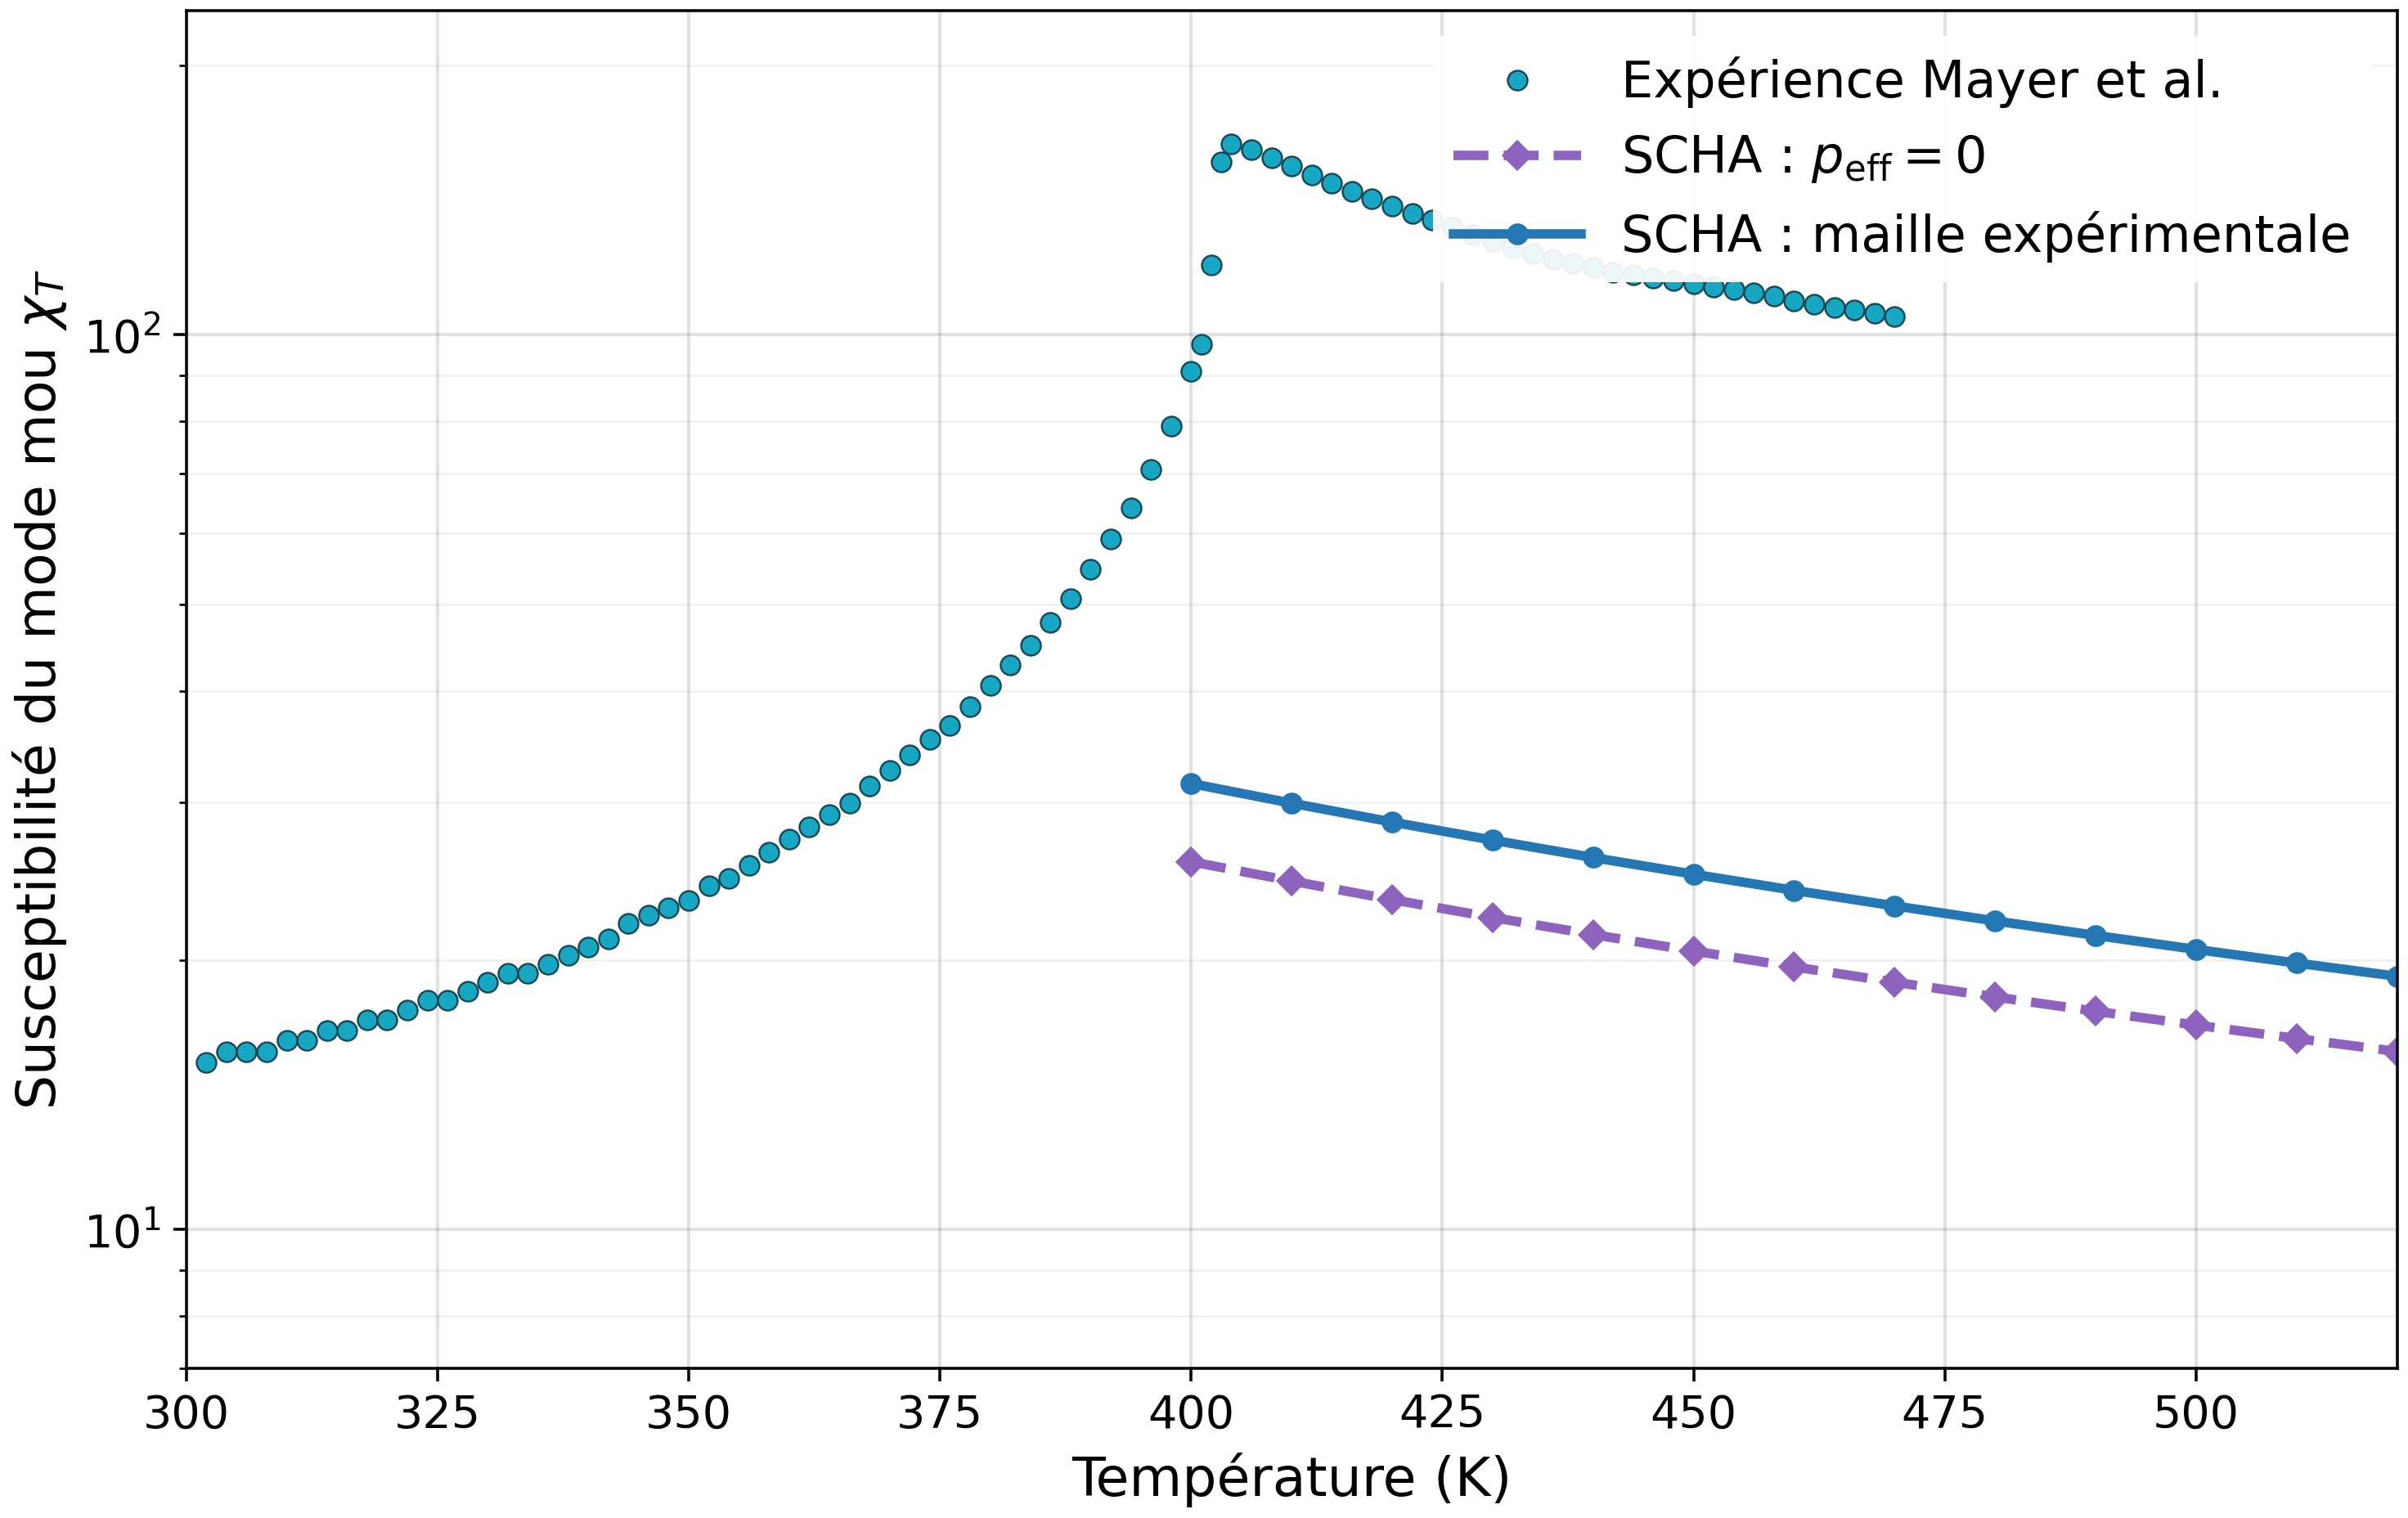
\includegraphics[width=\linewidth,height=1.46cm,keepaspectratio]
            {mayer_scha_slide_simplified.png}}
        \vspace{0.05cm}

        {\color{WarmGold}\bfseries Pourquoi dépasser la SCHA ?\par}
        \vfill
        \hyperlink{qa-post-scha}{\beamergotobutton{Revoir la slide 21}}
      \end{minipage}
  \end{columns}
\end{frame}

% =============================================================================
% ANNEXES TECHNIQUES
% =============================================================================

\appendix

\begin{frame}{Annexe --- références principales I}
  \small
  \begin{itemize}\setlength\itemsep{0.28cm}
    \item W. Zhong, D. Vanderbilt, K. M. Rabe, « Phase Transitions in BaTiO$_3$ from First Principles », \textit{Phys. Rev. Lett.} 73, 1861 (1994). \href{https://doi.org/10.1103/PhysRevLett.73.1861}{doi:10.1103/PhysRevLett.73.1861}
    \item W. Zhong, D. Vanderbilt, K. M. Rabe, « First-principles theory of ferroelectric phase transitions for perovskites », \textit{Phys. Rev. B} 52, 6301 (1995). \href{https://doi.org/10.1103/PhysRevB.52.6301}{doi:10.1103/PhysRevB.52.6301}
    \item T. Nishimatsu et al., « Fast molecular-dynamics simulation for ferroelectric thin-film capacitors », \textit{Phys. Rev. B} 78, 104104 (2008). \href{https://doi.org/10.1103/PhysRevB.78.104104}{doi:10.1103/PhysRevB.78.104104}
    \item T. Nishimatsu et al., « First-principles accurate total-energy surfaces for polar structural distortions », \textit{Phys. Rev. B} 82, 134106 (2010). \href{https://doi.org/10.1103/PhysRevB.82.134106}{doi:10.1103/PhysRevB.82.134106}
    \item T. Nishimatsu et al., « Molecular Dynamics Simulations of Chemically Disordered (Ba,Sr)TiO$_3$ », \textit{J. Phys. Soc. Jpn.} 85, 114714 (2016). \href{https://doi.org/10.7566/JPSJ.85.114714}{doi:10.7566/JPSJ.85.114714}
  \end{itemize}
\end{frame}

\begin{frame}{Annexe --- références principales II}
  \small
  \begin{itemize}\setlength\itemsep{0.19cm}
    \item J. H. Barrett, « Dielectric Constant in Perovskite Type Crystals », \textit{Phys. Rev.} 86, 118 (1952). \href{https://doi.org/10.1103/PhysRev.86.118}{doi:10.1103/PhysRev.86.118}
    \item K. A. Müller, H. Burkard, « SrTiO$_3$: An intrinsic quantum paraelectric below 4 K », \textit{Phys. Rev. B} 19, 3593 (1979). \href{https://doi.org/10.1103/PhysRevB.19.3593}{doi:10.1103/PhysRevB.19.3593}
    \item K. Wieczorek et al., « Electrostrictive and Piezoelectric Effect in BaTiO$_3$ and PbZrO$_3$ », \textit{Ferroelectrics} 336, 61 (2006). \href{https://doi.org/10.1080/00150190600695743}{doi:10.1080/00150190600695743}
    \item F. Mayer et al., « Improved description of the potential energy surface in BaTiO$_3$ by anharmonic phonon coupling », \textit{Phys. Rev. B} 106, 064108 (2022). \href{https://doi.org/10.1103/PhysRevB.106.064108}{doi:10.1103/PhysRevB.106.064108}
    \item R. Bianco et al., « Free Energy Curvature and Temperature-Dependent Anharmonic Phonons in the SCHA », \textit{Phys. Rev. B} 96, 014111 (2017). \href{https://doi.org/10.1103/PhysRevB.96.014111}{doi:10.1103/PhysRevB.96.014111}
    \item O. Auciello et al., \textit{J. Electroceram.} 12, 119--131 (2004). \href{https://doi.org/10.1023/B:JECR.0000034006.59246.5e}{doi:10.1023/B:JECR.0000034006.59246.5e}
  \end{itemize}
\end{frame}

% État interactif de la slide 13, placé hors de la navigation séquentielle.
\newcounter{slidethirteensavedframenumber}
\newcounter{slidethirteensavedsection}
\setcounter{slidethirteensavedframenumber}{\value{framenumber}}
\setcounter{slidethirteensavedsection}{\value{section}}
\begingroup
  \setcounter{framenumber}{13}
  \setcounter{section}{2}
  \def\insertsectionhead{Modèle et méthode de calcul}
  \setbeamerfont{frametitle}{series=\bfseries,size=\fontsize{16.5}{19}}
  \newcommand{\slidethirteenpopupcontent}{%
    \begin{tikzpicture}[remember picture,overlay]
      \fill[white,opacity=0.94]
        ([yshift=-1.84cm]current page.north west)
        rectangle
        ([yshift=0.35cm]current page.south east);
      \node[draw=bordeauCS,fill=white,rounded corners=4pt,line width=1.2pt,
        minimum width=11.85cm,minimum height=5.55cm]
        (hamiltonianpanel) at ([yshift=-0.28cm]current page.center) {};
      \node at (hamiltonianpanel.center) {%
        \hyperlink{slide13-closed}{\phantom{\rule{11.45cm}{5.25cm}}}};
      \node[text width=11.25cm,align=center,inner sep=0pt]
        at ([yshift=0.02cm]hamiltonianpanel.center) {%
        {\color{bordeauCS}\bfseries\fontsize{12.2}{14.2}\selectfont
          Hamiltonien effectif complet}\hfill
        {\color{Slate}\fontsize{7.0}{8.2}\selectfont cliquer sur le panneau pour fermer}\par
        \vspace{0.10cm}
        {\fontsize{6.25}{7.35}\selectfont
        \(\displaystyle
          \begin{aligned}
          H_{\mathrm{eff}}(p)={}&
          \sum_i\left(
            {\color{CSOrange}
              \frac{\bm\pi_{u,i}^{\,2}}{2M^*}
              +\frac12\alpha_0|\bm u_i|^2
              +\frac14\beta_{\alpha\beta\gamma\delta}
                u_i^\alpha u_i^\beta u_i^\gamma u_i^\delta
              +\frac16\gamma_{\alpha\beta\gamma\cdots\zeta}
                u_i^\alpha\cdots u_i^\zeta
              +\frac18\rho_{\alpha\beta\gamma\cdots\lambda}
                u_i^\alpha\cdots u_i^\lambda}
          \right)\\[-0.03cm]
          &+{\color{CSOrange}\frac12\sum_{i\ne j}u_i^\alpha
            \bigl(D_{ij}^{\alpha\beta}+J_{ij}^{\alpha\beta}\bigr)u_j^\beta
          }
          +{\color{HomStrainPurple}\frac{N}{2}\eta_\ell^{\mathrm{hom}}\mathcal B_{\ell m}
            \eta_m^{\mathrm{hom}}}\\[-0.03cm]
          &+{\color{InhomStrainGreen}\sum_i\frac{\bm\pi_{w,i}^{\,2}}{2M_w}}
          +{\color{InhomStrainGreen}\frac12\sum_{i,j}w_i^\alpha
            \Phi_{ij,\alpha\beta}^{\mathrm{elas,inh}}w_j^\beta}
          +\frac12\sum_{i,\ell,\alpha,\beta}B_{\ell\alpha\beta}
            \Bigl[{\color{HomStrainPurple}\eta_\ell^{\mathrm{hom}}}
            +{\color{InhomStrainGreen}\eta_{i,\ell}^{\mathrm{inh}}(\bm w)}\Bigr]
            u_i^\alpha u_i^\beta
          +\textcolor{PressureBlue}{p\Omega}.
          \end{aligned}
        \)\par}
        \vspace{0.08cm}
        {\fontsize{6.5}{7.6}\selectfont
          {\color{CSOrange}mode polaire}\quad
          {\color{HomStrainPurple}strain homogène}\quad
          {\color{InhomStrainGreen}strain inhomogène}\quad
          {\color{PressureBlue}pression externe}.}
      };
    \end{tikzpicture}%
  }
  \begin{frame}[label=slide13-popup,noframenumbering]
    \frametitle{L'anharmonicité génère la boucle qui corrige la rigidité}
    \slidethirteenpopupcontent
  \end{frame}
\endgroup
\setcounter{framenumber}{\value{slidethirteensavedframenumber}}
\setcounter{section}{\value{slidethirteensavedsection}}

\end{document}
